\documentclass[]{book}
\usepackage[]{mathpazo}
\usepackage{amssymb,amsmath}
\usepackage{ifxetex,ifluatex}
\usepackage{fixltx2e} % provides \textsubscript
\ifnum 0\ifxetex 1\fi\ifluatex 1\fi=0 % if pdftex
  \usepackage[T1]{fontenc}
  \usepackage[utf8]{inputenc}
\else % if luatex or xelatex
  \ifxetex
    \usepackage{mathspec}
  \else
    \usepackage{fontspec}
  \fi
  \defaultfontfeatures{Ligatures=TeX,Scale=MatchLowercase}
\fi
% use upquote if available, for straight quotes in verbatim environments
\IfFileExists{upquote.sty}{\usepackage{upquote}}{}
% use microtype if available
\IfFileExists{microtype.sty}{%
\usepackage{microtype}
\UseMicrotypeSet[protrusion]{basicmath} % disable protrusion for tt fonts
}{}
\usepackage[margin=1in]{geometry}
\usepackage{hyperref}
\PassOptionsToPackage{usenames,dvipsnames}{color} % color is loaded by hyperref
\hypersetup{unicode=true,
            pdftitle={Guide to R package},
            pdfauthor={author},
            colorlinks=true,
            linkcolor=red,
            citecolor=red,
            urlcolor=blue,
            breaklinks=true}
\urlstyle{same}  % don't use monospace font for urls
\usepackage{natbib}
\bibliographystyle{apalike}
\usepackage{color}
\usepackage{fancyvrb}
\newcommand{\VerbBar}{|}
\newcommand{\VERB}{\Verb[commandchars=\\\{\}]}
\DefineVerbatimEnvironment{Highlighting}{Verbatim}{commandchars=\\\{\}}
% Add ',fontsize=\small' for more characters per line
\usepackage{framed}
\definecolor{shadecolor}{RGB}{248,248,248}
\newenvironment{Shaded}{\begin{snugshade}}{\end{snugshade}}
\newcommand{\KeywordTok}[1]{\textcolor[rgb]{0.13,0.29,0.53}{\textbf{#1}}}
\newcommand{\DataTypeTok}[1]{\textcolor[rgb]{0.13,0.29,0.53}{#1}}
\newcommand{\DecValTok}[1]{\textcolor[rgb]{0.00,0.00,0.81}{#1}}
\newcommand{\BaseNTok}[1]{\textcolor[rgb]{0.00,0.00,0.81}{#1}}
\newcommand{\FloatTok}[1]{\textcolor[rgb]{0.00,0.00,0.81}{#1}}
\newcommand{\ConstantTok}[1]{\textcolor[rgb]{0.00,0.00,0.00}{#1}}
\newcommand{\CharTok}[1]{\textcolor[rgb]{0.31,0.60,0.02}{#1}}
\newcommand{\SpecialCharTok}[1]{\textcolor[rgb]{0.00,0.00,0.00}{#1}}
\newcommand{\StringTok}[1]{\textcolor[rgb]{0.31,0.60,0.02}{#1}}
\newcommand{\VerbatimStringTok}[1]{\textcolor[rgb]{0.31,0.60,0.02}{#1}}
\newcommand{\SpecialStringTok}[1]{\textcolor[rgb]{0.31,0.60,0.02}{#1}}
\newcommand{\ImportTok}[1]{#1}
\newcommand{\CommentTok}[1]{\textcolor[rgb]{0.56,0.35,0.01}{\textit{#1}}}
\newcommand{\DocumentationTok}[1]{\textcolor[rgb]{0.56,0.35,0.01}{\textbf{\textit{#1}}}}
\newcommand{\AnnotationTok}[1]{\textcolor[rgb]{0.56,0.35,0.01}{\textbf{\textit{#1}}}}
\newcommand{\CommentVarTok}[1]{\textcolor[rgb]{0.56,0.35,0.01}{\textbf{\textit{#1}}}}
\newcommand{\OtherTok}[1]{\textcolor[rgb]{0.56,0.35,0.01}{#1}}
\newcommand{\FunctionTok}[1]{\textcolor[rgb]{0.00,0.00,0.00}{#1}}
\newcommand{\VariableTok}[1]{\textcolor[rgb]{0.00,0.00,0.00}{#1}}
\newcommand{\ControlFlowTok}[1]{\textcolor[rgb]{0.13,0.29,0.53}{\textbf{#1}}}
\newcommand{\OperatorTok}[1]{\textcolor[rgb]{0.81,0.36,0.00}{\textbf{#1}}}
\newcommand{\BuiltInTok}[1]{#1}
\newcommand{\ExtensionTok}[1]{#1}
\newcommand{\PreprocessorTok}[1]{\textcolor[rgb]{0.56,0.35,0.01}{\textit{#1}}}
\newcommand{\AttributeTok}[1]{\textcolor[rgb]{0.77,0.63,0.00}{#1}}
\newcommand{\RegionMarkerTok}[1]{#1}
\newcommand{\InformationTok}[1]{\textcolor[rgb]{0.56,0.35,0.01}{\textbf{\textit{#1}}}}
\newcommand{\WarningTok}[1]{\textcolor[rgb]{0.56,0.35,0.01}{\textbf{\textit{#1}}}}
\newcommand{\AlertTok}[1]{\textcolor[rgb]{0.94,0.16,0.16}{#1}}
\newcommand{\ErrorTok}[1]{\textcolor[rgb]{0.64,0.00,0.00}{\textbf{#1}}}
\newcommand{\NormalTok}[1]{#1}
\usepackage{longtable,booktabs}
\usepackage{graphicx,grffile}
\makeatletter
\def\maxwidth{\ifdim\Gin@nat@width>\linewidth\linewidth\else\Gin@nat@width\fi}
\def\maxheight{\ifdim\Gin@nat@height>\textheight\textheight\else\Gin@nat@height\fi}
\makeatother
% Scale images if necessary, so that they will not overflow the page
% margins by default, and it is still possible to overwrite the defaults
% using explicit options in \includegraphics[width, height, ...]{}
\setkeys{Gin}{width=\maxwidth,height=\maxheight,keepaspectratio}
\setlength{\emergencystretch}{3em}  % prevent overfull lines
\providecommand{\tightlist}{%
  \setlength{\itemsep}{0pt}\setlength{\parskip}{0pt}}
\setcounter{secnumdepth}{5}
% Redefines (sub)paragraphs to behave more like sections
\ifx\paragraph\undefined\else
\let\oldparagraph\paragraph
\renewcommand{\paragraph}[1]{\oldparagraph{#1}\mbox{}}
\fi
\ifx\subparagraph\undefined\else
\let\oldsubparagraph\subparagraph
\renewcommand{\subparagraph}[1]{\oldsubparagraph{#1}\mbox{}}
\fi

%%% Use protect on footnotes to avoid problems with footnotes in titles
\let\rmarkdownfootnote\footnote%
\def\footnote{\protect\rmarkdownfootnote}

%%% Change title format to be more compact
\usepackage{titling}

% Create subtitle command for use in maketitle
\newcommand{\subtitle}[1]{
  \posttitle{
    \begin{center}\large#1\end{center}
    }
}

\setlength{\droptitle}{-2em}

  \title{Guide to R package}
    \pretitle{\vspace{\droptitle}\centering\huge}
  \posttitle{\par}
    \author{author}
    \preauthor{\centering\large\emph}
  \postauthor{\par}
      \predate{\centering\large\emph}
  \postdate{\par}
    \date{2018-09-14}

\usepackage{booktabs}
\usepackage{longtable}
\usepackage{array}
\usepackage{multirow}
\usepackage[table]{xcolor}
\usepackage{wrapfig}
\usepackage{float}
\usepackage{colortbl}
\usepackage{pdflscape}
\usepackage{tabu}
\usepackage{threeparttable}
\usepackage{threeparttablex}
\usepackage[normalem]{ulem}
\usepackage{makecell}

\usepackage{amsthm}
\newtheorem{theorem}{Theorem}[chapter]
\newtheorem{lemma}{Lemma}[chapter]
\theoremstyle{definition}
\newtheorem{definition}{Definition}[chapter]
\newtheorem{corollary}{Corollary}[chapter]
\newtheorem{proposition}{Proposition}[chapter]
\theoremstyle{definition}
\newtheorem{example}{Example}[chapter]
\theoremstyle{definition}
\newtheorem{exercise}{Exercise}[chapter]
\theoremstyle{remark}
\newtheorem*{remark}{Remark}
\newtheorem*{solution}{Solution}
\begin{document}
\maketitle

{
\hypersetup{linkcolor=black}
\setcounter{tocdepth}{2}
\tableofcontents
}
\chapter{Introduction}\label{part_1}

\begin{quote}
\emph{One of the greatest advantages of R: getting your work done better
and in less time.}

--- Frank Harrell, Biostatistics, Vanderbilt University
\end{quote}

This chapter presents basic information related to R software and is
aimed at readers who have never heard about R, do not know how to work
with it, or are perhaps not sure whether R is worth the effort.

We will begin by presenting the advantages of R. Next, we will discuss
its history and development, followed by a presentation of what it feels
like to work with R. We will use a simple example to show you how to
read data, process it and create plots. After that, we will find out how
to configure the environment and how to install its necessary
components. Finally, we will list sources with further information
related to R.

\section{Data science, or why we should learn R}\label{part_11}

Data science is a dynamically growing discipline which combines data
analysis and programming. There is an ever-increasing need for people
who can analyse newly emerging data streams. In order to keep pace with
the contemporary digital tsunami, we need robust tools to analyse data.
One of such tools is the R language.

There are numerous programming languages, but R allows you to analyse
data much quicker than any other language. You can go to
\url{http://bit.ly/2fXfWV2} (Video Introduction to R by Microsoft) to
see a 90-second video which presents the potential of R software.

Why? R was created to facilitate working with data. The R language is a
dialect of the S language developed by John Chambers from Bell Labs
around 1976. The S language was developed for interactive data analysis.
Numerous solutions were introduced to it to simplify data processing.

The first version of R was developed in 1991 by Robert Gentleman and
Ross Ihaka (also known as R\&R) who worked in the Department of
Statistics at the University of Auckland. Initially, the R package was
meant as a teaching resource at that university. At the same time, it
was an open project, which is why it quickly gained in popularity. Since
1997, over twenty people worked on the development of R, thus
constituting the so-called core team. The team comprises experts from
various fields (statistics, mathematics, numerical methods, and computer
science in a broad sense) from all over the world. The number of people
developing R grew quickly. Today, the project is developed by ``The
Foundation for Statistical Computing'' that has hundreds of members.
Apart from that, there are thousands of people all around the world who
share their own packages with various functions. The number of R
libraries grows rapidly. In 2016, there were over 10,000 packages in the
main CRAN repository (see Figure \ref{fig:figs}). Apart from that, there
are thousands of packages that are private or placed in other
repositories.

\begin{Shaded}
\begin{Highlighting}[]
\KeywordTok{plot}\NormalTok{(}\DecValTok{1}\OperatorTok{:}\DecValTok{5}\NormalTok{)}
\end{Highlighting}
\end{Shaded}

\begin{figure}

{\centering 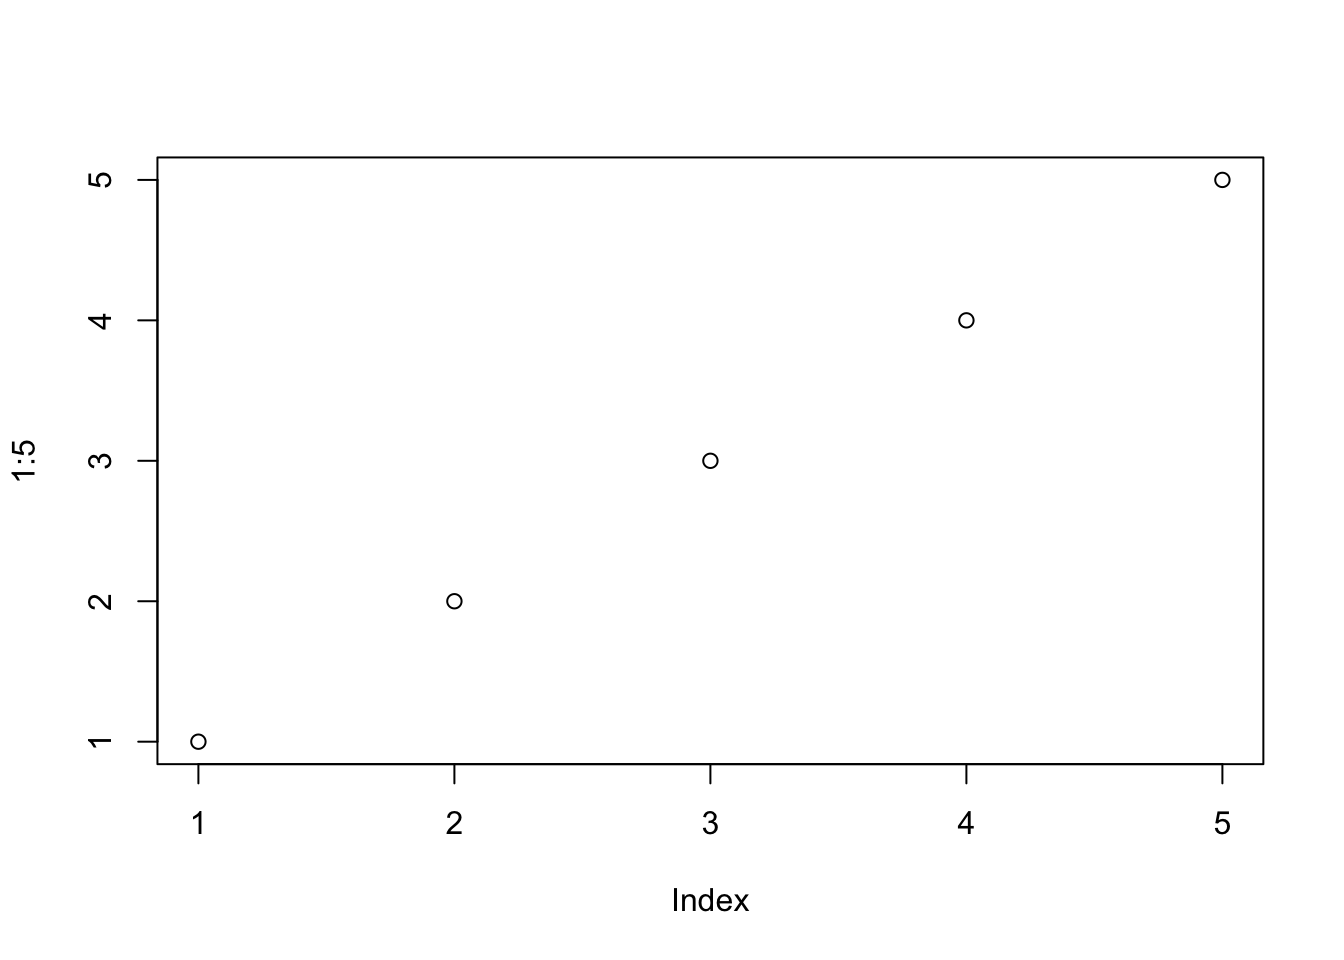
\includegraphics{Przewodnik_gitbook_80_files/figure-latex/figs-1} 

}

\caption{plot bar}\label{fig:figs}
\end{figure}

To tylko robocze odwołanie do rozdziału
\protect\hyperlink{part_121}{1.2.1}

To tylko robocze odwołanie do artykułu \citep{hs1986} zamieszczonego w
bibliografii.

\begin{equation}
f\left(k\right)=\binom{n}{k}p^k\left(1-p\right)^{n-k}
\label{eq:binom}
\end{equation}

To tylko robocze odwołanie do równania \eqref{eq:binom}.

R is a GNU project based on the GNU GPL license, which means it is free
of charge for both educational and commercial use. More information
about GNU GPL can be found at {[}53{]}. The R platform has excellent
documentation available as PDF files or HTML pages. The documentation is
mostly in English, but some files have other language versions as well.

The R language has been developed for people dealing with data from the
very beginning. This is why it was frequently treated as a
domain-specific language (DSL) by many computer scientists rather than a
full-featured language. As time went by, however, the capabilities of R
expanded and more solutions outside the field of data analysis appeared.
Today, R is one of the most popular programming languages.

One evidence of this is the ranking created based on the votes by the
IEEE committee members (Institute of Electrical and Electronics
Engineer). In 2016, R ranked as the fifth most popular language,
outrunning such languages as PHP or JavaScript.

There are multiple reasons behind the popularity of R. Below, we present
those we consider the most significant ones.

\begin{itemize}
\item
  Because of its elasticity, R is nowadays the most basic language used
  when teaching statistics and data analysis, present at practically any
  good university.
\item
  R software allows us to create and share packages that contain new
  functions. Currently, there are over 10,000 packages for multiple
  purposes, such as rgl -- for 3D graphics, lima -- for microarray data
  analysis, seqinr -- for genomics data analysis, psy -- with
  statistical functions commonly used in psychometry, geoR -- with
  geostatistical functions, Sweave -- for report generation using LaTeX,
  and many others. Everyone can create and share their own packages.
\item
  The R software allows us to use functions written in other languages
  (C, C++, Fortran). What is more, we can execute functions available in
  R from other languages (Java, C, C++, Statistica packages, SAS, and
  many others). Thanks to that, we can write most of our application in
  Java, and use R as a big external library with statistical functions.
\item
  R software facilitates creating high-quality plots, which is of vital
  importance when presenting results. Even with their default settings,
  those plots look much better than their counterparts in other
  packages.
\end{itemize}

More about the history and development of R can be found at
\url{http://bit.ly/2domniT} (``R Programming'' at
\url{https://www.coursera.org/}).

\section{What working with R looks like}\label{part1_2}

We work with R in an interactive way. The R software itself is often
associated with a console that has a blinking cursor used to enter
commands and read results.

We wanted to reflect this work style in this book, which is why we
present sample code alongside the output generated by the software. Both
R instructions and their results are presented against a grey background
so that you can find them quickly. Results are presented on lines that
start with a double hash sign (\#\#).

For example, the \texttt{substr()} function cuts out a substring with
the coordinates provided in the parentheses. When you run the R
software, you only need to type the instruction below to see the result
in the same console window. Here, the result will be a string containing
a single \texttt{R} letter.

\begin{Shaded}
\begin{Highlighting}[]
\KeywordTok{substr}\NormalTok{(}\StringTok{"What is supeR?"}\NormalTok{, }\DataTypeTok{start =} \DecValTok{13}\NormalTok{, }\DataTypeTok{stop =} \DecValTok{13}\NormalTok{)}
\end{Highlighting}
\end{Shaded}

\begin{verbatim}
## [1] "R"
\end{verbatim}

When we write about functions, packages, and language elements, we use a
\texttt{fixed-width\ font}. Some key English terms are written in
italics. When we first mention a function name from an untypical
package, we mention the package name.

The \texttt{ggplot2::qplot()} notation signifies function
\texttt{qplot()} in the \texttt{ggplot2} package. Sometimes, there are
multiple functions in different packages that have the same name. In
this case, we can precisely specify the function by providing the name
of the package in front of it. When we need to install or turn on an
uncommon package to use a given function, it is better to know which
package offers the given function. At the end of this book, there is an
index of functions -- they are presented both alphabetically and by
packages.

\hypertarget{part_121}{\subsection{Example: Poland in the FIFA
ranking}\label{part_121}}

Let us find out what ``serious'' work with R looks like based on the
example below.

\begin{itemize}
\item
  We will use some functions from the \texttt{rvest} package to directly
  read Poland's FIFA rank from Wikipedia.
\item
  We will use some functions from the \texttt{tidyr} and \texttt{dplyr}
  packages to transform the data into the appropriate form.
\item
  We will use some functions from the \texttt{ggplot2} package to
  graphically present the data.
\end{itemize}

The entire R code which deals with those 3 stages is quite short and
easy to analyse in a step-by-step manner. Some elements may seem
familiar while others will appear surprising. We will explain the
meaning of each element in subsequent sections.

\begin{quote}
All R instructions contained in this book can be downloaded from
\url{http://biecek.pl/R}. The R instructions provided will always yield
the same results. The only exception from this rule are some plots that
have been modified to increase their readability in print.
\end{quote}

\subsubsection{Loading data}\label{part_1211}

The code snippet below loads a data table from the Polish version of
\emph{Poland national football team} available on Wikipedia. We used
\texttt{rvest}, a package which is very useful for downloading data from
websites.

There are multiple tables on the site we are interested in. We get them
all, and then choose the one with 14 columns. Having loaded the data, we
show the first 6 rows.

\begin{verbatim}
library("rvest")
wikiPL <- "https://pl.wikipedia.org/wiki/Reprezentacja_Polski_w_piłce_nożnej_mężczyzn"
webpage <- read_html(wikiPL)
table_links <- html_nodes(webpage, '.wikitable')
tables <- html_table(table_links, fill=TRUE)
FIFA_table <- which(sapply(tables, ncol) == 14)
tab <- tables[[FIFA_table]]
head(tab)
\end{verbatim}

\subsubsection{Data transformation}\label{part_1212}

Another step after loading the data is cleaning and transforming it. To
that end, we can use functions from the \texttt{tidyr} and
\texttt{dplyr} packages. We will explain them in detail shortly. For the
time being, we will provide an abbreviated explanation.

We change the data from the wide format, in which months are stored in
different columns, into the narrow format, where all months are stored
in a single column. Then, we change Roman numerals used for months into
Arabic numerals. At this point, our data is ready to be presented
graphically.

\begin{verbatim}
library("tidyr")
library("dplyr")
colnames(tab)[2:13] <- 1:12
data_long <- gather(tab[,1:13], Month, Rank, -Year)
data_long <- mutate(data_long,
                    Position = as.numeric(Position),
                    Month = as.numeric(Month))
head(data_long, 3)
\end{verbatim}

\subsubsection{Graphical data presentation}\label{part_1213}

Now that we have loaded the data, it is time we looked at it. We can use
the \texttt{ggplot2} package for graphical presentation purposes. Below,
we present instructions that will generate the chart visible in Figure
1.3, which is called a box plot. It presents the minimal, maximal,
mid-range and interquartile rank of Poland in each year of the ranking.
We can see when the most prominent changes took place and when Poland
reached its best ranks.

\begin{verbatim}
library("ggplot2")
ggplot(data_long, aes(factor(Year), Rank)) +
geom_boxplot() + ggtitle("Rank of Poland in FIFA Ranking")
\end{verbatim}

\section{Setting up the environment}\label{part_13}

To enjoy a convenient R environment, we should follow the three steps
below.

\begin{itemize}
\item
  Install the basic R environment, which comprises an interpreter and a
  basic set of packages. This set alone offers enormous capabilities. It
  will be enough for most users to analyse data, draw plots and perform
  other typical tasks.
\item
  Install RStudio. It is a tool which facilitates working with the R
  software. It is not the only R editor out there, but seems to be the
  best solution. Similarly to R itself, the basic version of RStudio is
  free of charge.
\item
  Install additional packages with useful functions. There are over
  7,000 packages available now! You do not have to install them all at
  once. You will sometimes need new functions from new packages as you
  work with R, and it is only then that you should install them.
\end{itemize}

Below, we present a short summary related to each installation stage.

\subsection{Installing basic R environment}\label{part_131}

The source and binary R files are available for most operating systems,
including all Linux and Unix distributions, Windows 95 or higher, and
Mac OS.

At the time of this writing, the latest R version is 3.3.2. Each year in
April, there is another major 3.x version appearing, which means that we
will soon enjoy version 3.4.0. During the year, further subversions are
released as need be. R is being developed quickly and we should update
it at least once a year to get its latest version.

In order to install R, go to \url{https://cran.r-project.org/}, choose
the operating system and download the binary file. The installation
itself is as simple as clicking Next a few times. You can have a few
versions of R installed at the same time. Keeping older versions of R
may be useful when we want to reproduce the exactly same results in the
future.

If you install R on a less typical platform, you can use the
installation manual available at {[}49{]}.

\begin{quote}
One useful feature of the R environment is that you can run it without
installation. This means you can copy your R environment onto a CD,
pendrive or external hard drive and run it on any other computer.
\end{quote}

It is hard to estimate the minimal system requirements for R. Its basic
version runs without problems on older computers with 256 MB of RAM,
Pentium processors and a few dozen MB of space on the hard drive.
However, even though the basic version is ``lightweight'', the
installation of additional packages may require a few more GBs of RAM or
hard drive space. Packages with big genomic data are particularly
``heavy-weight''.

\begin{quote}
Those using R for compute-intensive analyses should rather use the R
version for OS X, Linux or Unix. These systems manage memory more
efficiently, which means that R works (slightly) faster. Unix-based
systems also provide additional tools that allow multiple threads and
other system mechanisms (such us \texttt{fork()}).
\end{quote}

\subsection{Installing RStudio}\label{part_132}

You can work with the basic R software alone, but working with an editor
is much more convenient, especially when R is our main tool at work.
Currently, the best editor available free of charge is RStudio -- a tool
developed by a company under the same name. This editor is available for
Windows, Linux and OS X alike, supports many advanced packages and
functions of R.

RStudio is a tool which makes working with R easier. It is an editor,
version manager, and debugger that makes creating packages, applications
or reports easier. You can live without it, but it certainly helps much.
The latest version of RStudio Desktop can be found at
\url{https://www.rstudio.com/}.

An example screenshot from the program is shown in Figure 1.5.

RStudio is very intuitive. Some of its interesting functions are:

\begin{itemize}
\item
  Ability to automatically send the whole script or a piece of it to the
  R console. After selecting a given code snippet and pressing
  \texttt{Ctrl-Enter}, it will be executed in the R console.
\item
  Ability to manage multiple files and/or projects.
\item
  Support for \texttt{knitr}, \texttt{Sweave} and \texttt{shiny}
  packages, easy navigation among code fragments.
\item
  Support for R Notebooks, which allows interactive work with reports
  and running/updating code snippets.
\item
  Showing objects (names, classes, dimensions) available in the
  namespace.
\item
  Editor for data, functions and other R objects. When we click the name
  of a set present in the namespace, we can edit that object. It is
  often more convenient than using \texttt{fix()} or \texttt{edit()}.
\item
  A simplified way to load data using a graphical interface.
\item
  Highlighting keywords and function names.
\item
  Contextual name auto-completion for functions, variables, properties,
  function arguments (when we start typing names, a list with matches
  appears).
\item
  Showing/hiding the code of functions or loops.
\item
  Support for creating and testing new packages.
\item
  Closing open brackets and quotes along with intelligent content
  highlighting.
\item
  Intelligent insertion of indentation combined with syntax recognition
  (i.e.~indentation is added in loops, functions, etc.).
\item
  Interactive debugger.
\end{itemize}

RStudio Server is an interesting extension of RStudio Desktop. After
installing it on a server, we can use R via our web browser. With the
paid version, multiple users may open R at the same time.

Work in RStudio is much easier when you know some basic shortcuts. Below
are those I personally find the most interesting. A very good
description of RStudio alongside all keyboard shortcuts can be found at
\url{http://bit.ly/2d4B0Ix} (so-called RStudio IDE cheatsheets). In the
description below, \texttt{Ctrl/Cmd} means \texttt{Ctrl} for
Windows/Linux and \texttt{Cmd} for OS X.

\begin{itemize}
\item
  \texttt{Ctrl/Cmd+Shift+C}, comment a line or multiple lines.
\item
  \texttt{Ctrl/Cmd+Enter}, execute the highlighted code in the console.
\item
  \texttt{Ctrl/Cmd+Up}, show the history of commands.
\item
  \texttt{Ctrl+L}, clear the console.
\item
  \texttt{Ctrl+1-9}, switch between application windows.
\item
  \texttt{Tab}, autocomplete code -- a very useful feature indeed.
\item
  \texttt{Ctrl/Cmd+Shift+K}, compile the current document.
\end{itemize}

\subsection{Installing additional packages}\label{part_133}

Once we have the basic R environment in place, we already have access to
various features. The real power, however, lies in the thousands of
additional packages that contain further thousands of functions.

In order to use additional packages, we should follow these two steps:

\begin{enumerate}
\def\labelenumi{\arabic{enumi}.}
\item
  Install a new package on the hard drive. You only need to do this
  once, the necessary files will be copied into the directory with
  packages. You can check the path to the directory with
  \texttt{.libPaths()}.
\item
  Turn on the installed package in an active R session. This step must
  be performed every time we run the R environment. This will make the
  functions and datasets from the package available in the current
  session.
\end{enumerate}

There are a few ways to install packages. We usually install them from
the official CRAN repository (The Comprehensive R Archive Network). If
the package we are interested in is available in CRAN, we can install it
using \texttt{install.packages()}.

For instance, the instruction below installs the \texttt{Przewodnik}
package (Polish for \emph{Guide}) directly from the CRAN repository
alongside all the dependencies and datasets that we will use in this
book. In order to install it, you only need to type the following code
in the R console:

\begin{verbatim}
install.packages("Przewodnik")
\end{verbatim}

Or choose \texttt{Tools/Install\ packages...} in RStudio.

Some packages are missing from the CRAN repository or are available in
some older versions. For example, packages in CRAN are required to be 10
MB in size at most. Because of this limitation, greater packages must be
stored elsewhere, typically in GitHub repositories. In order to install
packages from GitHub, you can use the
\texttt{devtools:install\_github()} instruction.

For example, if you want to install the latest version of our
\texttt{Przewodnik} package from the \texttt{pbiecek} Github repository,
you can use:

\begin{verbatim}
devtools::install_github("pbiecek/PrzewodnikPakiet")
\end{verbatim}

Apart from these two repositories, there are repositories for special
purposes. For instance, many packages used in bioinformatical analyses
can be found in the \texttt{Bioconductor} repository available at
\url{https://www.bioconductor.org/}.

When we install a new package with data, functions and auxiliary files,
they are stored on the hard drive of our computer. Before we can use
them, however, we need to turn the package on. Each time we run the R
platform, some basic packages such as \texttt{base}, \texttt{graphics}
or \texttt{stats} are loaded. In order to use additional functions or
datasets, we need to load (turn on) the package which contains them
(assuming that the package is already installed). We use the
\texttt{library()} instruction to turn packages on.

The instruction below turns on the \texttt{devtools} package. Once we
execute this instruction, we can use the package without the need to add
the \texttt{devtools::} prefix.

\begin{verbatim}
library("devtools")
\end{verbatim}

As we mentioned before, there are over 10,000 packages in the CRAN
repository. It is difficult to find the feature we need in such a broad
set. This is why we will use the following notation when using new
functions: \texttt{packageName::functionName()}.
\texttt{ggplot2::qplot()} means that the \texttt{qplot()} function can
be found in the \texttt{ggplot2} package. The index at the back of the
book lists all functions both alphabetically and grouped by packages.

If we know the name of a function and want to find out the package that
contains it, given that we do not have this book at hand, we can use the
\texttt{help.search()} function. It will search through all installed
packages and try to find the given name, or a function whose description
contains the given search phrase. More information about this function
and other means of searching information can be found in Section 1.4.

Once we have loaded the respective package, we can use its functions by
providing their names. We can also explicitly name the package a
function should come from. This might be useful when we have multiple
functions with the same name in different packages. For example, both
\texttt{epitools} and \texttt{vcd} packages contain an
\texttt{oddsratio()} function, but each of them works in a different
way. In order to specify the package, we can see the \texttt{::} or
\texttt{:::} operators. The \texttt{::} operator only allows referring
to public functions of a package, whereas the \texttt{:::} operator also
accepts references to private functions. Both lines of code below use
the \texttt{seq()} function from the \texttt{base} package. The second
method is useful when there are conflicting names of functions coming
from different packages.

\begin{verbatim}
seq(10)
base::seq(10)
\end{verbatim}

If we do not use the \texttt{::} operator while there are multiple
functions with the same name in different packages, R will use the
function from the package loaded most recently.

\section{Further information}\label{part_14}

In further parts of this book, we discuss libraries for data
transformation, statistical modelling or visualisations. We are sure,
however, that you will encounter problems or doubts not mentioned in
this book. Where can you look for other types of information?

The easiest and quickest way is to ask someone who knows the answer and
wants to help us.

It turns out that there is a large group of R enthusiasts who organise
recurring meetups with presentations. In Poland, there are currently
three major groups for R enthusiasts in three different cities. They
meet once a month, more or less.

\begin{itemize}
\item
  SER: Warsaw R User Group Meetups. \url{http://bit.ly/2epbNb9}.
\item
  eRka: Cracow Alternative for R Enthusiasts.
  \url{http://bit.ly/2fJ5N9o}.
\item
  PAZUR: Poznan R User Group. \url{http://bit.ly/2fKnTJE}.
\end{itemize}

There are also substantial groups for R users in Wroclaw, Lodz and other
cities where enthusiasts exchange information in data science meetups.

If we do not have an experienced friend, we can use the rich support
system offered by R. First of all, there are built-in R functions that
facilitate information lookup. The most useful ones among them are:

\begin{itemize}
\item
  The \texttt{help()} function which shows the welcome page of R's
  support system. The page describes the functions mentioned below in
  detail.
\item
  Functions \texttt{help("sort")} and \texttt{?sort} show a help page
  devoted to the \texttt{sort} function. Take a look at the example
  shown below as well. The format of descriptions is unified for ease of
  use. In RStudio, you can use the \texttt{F1} button to activate help
  for a specific function. Further help sections contain the following
  information: concise function description (\texttt{Description}
  section), function declarations (\texttt{Usage} section), explanation
  of all arguments (\texttt{Arguments} section), detailed function
  description (\texttt{Details} section), literature
  (\texttt{References} section), links to other functions
  (\texttt{See\ Also} section) as well as usage examples
  (\texttt{Examples} section). If we provide the \texttt{package}
  argument, we will get help related to the given package. For instance,
  \texttt{help(package=MASS)} will show the description of the
  \texttt{MASS} package.
\item
  \texttt{args("functionName")} shows the list of arguments of
  \texttt{functionName}.
\item
  \texttt{apropos("regression")} and \texttt{find("regression")} list
  functions (and objects) whose names contain the \texttt{regression}
  substring.
\item
  \texttt{example("plot")} runs a script with usage examples of
  \texttt{plot} function. Examples allow us to quickly find out how to
  use a function and what results we can expect.
\item
  \texttt{help.search("keyword")} browses the descriptions of functions
  contained in the packages we have installed and shows those functions
  where \texttt{keyWord} was found. In this case, \texttt{keyWord} may
  also contain multiple words or a phrase. The result list will
  additionally provide information about which package contains the
  functions it found.
\end{itemize}

The code below presents a sample session in R. We are looking for
information about the \texttt{plot()} function and functions to test
hypotheses. On the first line, we show help related to the \texttt{plot}
function, followed by usage examples. The next line shows all functions
with the ``test'' word in their names, and the last one shows functions
with the phrase ``normality test'' in their descriptions.

\begin{verbatim}
?plot
example(plot)
apropos("test")
help.search("normality test")
\end{verbatim}

The functions shown above look for information on a given topic by
browsing packages that are already installed on the hard drive. If this
proves insufficient (chances are we do not have packages with
potentially interesting functions installed), we can use the resources
available on the Internet. Particularly useful are the following
resources:

\begin{itemize}
\item
  Internet course in Polish called Pogromcy Danych (\emph{Data
  Busters}), available at \url{http://pogromcydanych.icm.edu.pl}. The
  course is divided into a dozen or so short blocks with exercises,
  allowing us to check our level of expertise.
\item
  StackExchange, a forum with numerous questions and hundreds of people
  eager to answer them. This forum often shows up in Google search
  results. It is available at \url{https://stackexchange.com/}.
\item
  Manuals devoted to various aspects of programming in R or data
  analyses in R. They are available directly from R's \texttt{Help}
  menu, and at \url{https://cran.r-project.org/manuals.html}.
\item
  \emph{R-bloggers}, and aggregator of blogs devoted to R, which is
  often a source of interesting information:
  \url{http://www.r-bloggers.com}.
\item
  Books devoted to R and data analysis using R. An up-to-date list of
  relevant books can be found at
  \url{https://www.r-project.org/doc/bib/R-books.html}.
\item
  Websites with questions and answers related to statistics and
  programming. For instance, \url{http://stats.stackexchange.com}
  (questions related to statistics) or
  \url{http://stackoverflow.com/questions/tagged/r} (questions related
  to programming).
\end{itemize}

There are multiple materials available in the Polish language on the
Internet. One of the first publications was \emph{Wprowadzenie do
środowiska R} by Łukasz Komsta {[}17{]}, but new resources appear every
year. A current list of Polish materials is available at
\url{https://pl.wikipedia.org/wiki/R}.

John Chambers {[}5{]} published a useful book for those who wish to
master the R language. If you want to learn statistical functions, in
turn, we recommend a book by Brian Everitt {[}8{]}. Both books deal with
the S language. However, it is almost identical with R from the user's
point of view. There are also numerous books, websites, and electronic
documents that deal with various aspects of the software and the R
language itself. At the end of 2007, a comprehensive book by Michael
Crawley {[}6{]} was published which is worth recommending. It presents
both R itself, as well as multiple statistical procedures implemented in
R. Besides, there are more and more books devoted to R software for
special purposes, some examples being: a book prepared by Paul Murell
devoted to graphics {[}21{]}, a book by Julian Faraway about linear
models {[}10{]}, or another work by Brian Everitt which deals with
statistics basics {[}9{]}. Springer has published over 45 books devoted
to R in a series called \texttt{Use\ R!}, and each of them deals with a
single subject, such as spatial data analysis, data visualisation,
social or genomic data etc.

\chapter{R Basics}\label{part_2}

This chapter presents basic information necessary to start working with
R. The first four sections introduce data loading from text files,
discuss key data structures in R, and present selected descriptive
statistics -- both numerical and graphical. We will go back to data
loading in Section 2.6, where we show how to load and save data in
various formats.

Next, we will discuss the \texttt{dplyr} and \texttt{tidyr} packages.
They allow us to perform most transformations and data aggregations such
as filtering, grouping and aggregate creation. The last subchapter
discusses how we can create automatic reports. It shows how we can use
the \texttt{knitr} package and RStudio to immediately create easily
readable reports.

\section{Loading data}\label{part_21}

The two most popular formats to store data are text files and
Excel/OpenOffice files. Both formats can be loaded into RStudio with
just a few mouse clicks. You only need to choose File/Import Dataset,
and a graphical interface for data import will appear -- see Figure 2.1.

If we encounter an untypical file formatting, we can use a few control
buttons to specify what the separator is, whether the first row contains
headers etc.

If we do not use RStudio, we can use function \texttt{read.table()} to
load data. An example of this function is given below.

File \url{http://www.biecek.pl/R/auta.csv} contains data on 2400 sales
offers for cars of different makes. This data is stored in a file with
.csv extension. Each offer contains 8 parameters which are separated
with semicolons in the text file.

A fragment of the file is shown below.

\begin{verbatim}
"Make";"Model";"Price";"HP";"Capacity";"Mileage";"Fuel";"
Production"
"Peugeot";"206";8799;60;1100;85000;"gasoline";2003
"Peugeot";"206";15500;60;1124;114000;"gasoline";2005
"Peugeot";"206";11900;90;1997;215000;"diesel";2003
"Peugeot";"206";10999;70;1868;165000;"diesel";2003
"Peugeot";"206";11900;70;1398;146000;"diesel";2005
"Peugeot";"206";19900;70;1398;86400;"diesel";2006
...
\end{verbatim}

The first argument of \texttt{read.table()} is the path to the file with
the data. The file can be located on a hard drive, or on the Internet.

The next two arguments in the function execution below specify that the
values in subsequent columns are separated with semicolons, and that the
first row contains variable names.

The result of function \texttt{read.table()} -- the table with data --
is assigned to the vehicles symbol using the \textless{}- operator.

\begin{Shaded}
\begin{Highlighting}[]
\NormalTok{vehicles <-}\StringTok{ }\KeywordTok{read.table}\NormalTok{(}\StringTok{"http://www.biecek.pl/R/auta.csv"}\NormalTok{,}
                       \DataTypeTok{sep =} \StringTok{";"}\NormalTok{, }\DataTypeTok{header =} \OtherTok{TRUE}\NormalTok{)}
\KeywordTok{head}\NormalTok{(vehicles)}
\end{Highlighting}
\end{Shaded}

\begin{verbatim}
##     Marka Model  Cena KM Pojemnosc Przebieg  Paliwo Produkcja
## 1 Peugeot   206  8799 60      1100    85000 benzyna      2003
## 2 Peugeot   206 15500 60      1124   114000 benzyna      2005
## 3 Peugeot   206 11900 90      1997   215000  diesel      2003
## 4 Peugeot   206 10999 70      1868   165000  diesel      2003
## 5 Peugeot   206 11900 70      1398   146000  diesel      2005
## 6 Peugeot   206 19900 70      1398    86400  diesel      2006
\end{verbatim}

The \texttt{head()} function shows the first 6 rows from the data set.
This function allows us to quickly find out what the table contains.

In Section 2.6 we discuss more methods of data loading using various
formats.

Once we have our data in place, it is time to work with it.

\section{Data structures}\label{part_22}

The data we are going to work with is usually stored as a table or a
vector of values. One of the basic operations on tables and vectors is
selecting a subset of rows, columns or values. More information about
various methods of data processing can be found in Section 2.5.

\subsection{Vectors}\label{part_221}

Vectors, or sequences of values of the same type, are the basic data
structure in R. We can create sequences of numbers, strings, or logical
values. For R, even a single number is a one-element vector.

Vectors can be created from smaller vectors using the \texttt{c()}
function.

\begin{Shaded}
\begin{Highlighting}[]
\KeywordTok{c}\NormalTok{(}\DecValTok{2}\NormalTok{, }\DecValTok{3}\NormalTok{, }\DecValTok{5}\NormalTok{, }\DecValTok{7}\NormalTok{, }\DecValTok{11}\NormalTok{, }\DecValTok{13}\NormalTok{, }\DecValTok{17}\NormalTok{)}
\end{Highlighting}
\end{Shaded}

\begin{verbatim}
## [1]  2  3  5  7 11 13 17
\end{verbatim}

One particular group of vectors are sequences of consecutive numbers.
The easiest way to create such sequences is by using the \texttt{:}
operator.

\begin{Shaded}
\begin{Highlighting}[]
\DecValTok{-3}\OperatorTok{:}\DecValTok{3}
\end{Highlighting}
\end{Shaded}

\begin{verbatim}
## [1] -3 -2 -1  0  1  2  3
\end{verbatim}

If we need sequences of numbers with a step value other than 1, we may
use the \texttt{seq()} function.

\begin{Shaded}
\begin{Highlighting}[]
\KeywordTok{seq}\NormalTok{(}\DataTypeTok{from =} \DecValTok{0}\NormalTok{, }\DataTypeTok{to =} \DecValTok{100}\NormalTok{, }\DataTypeTok{by =} \DecValTok{11}\NormalTok{)}
\end{Highlighting}
\end{Shaded}

\begin{verbatim}
##  [1]  0 11 22 33 44 55 66 77 88 99
\end{verbatim}

Many useful vectors are available in basic packages. Some examples are
month names or subsequent letters.

\begin{Shaded}
\begin{Highlighting}[]
\NormalTok{month.name}
\end{Highlighting}
\end{Shaded}

\begin{verbatim}
##  [1] "January"   "February"  "March"     "April"     "May"      
##  [6] "June"      "July"      "August"    "September" "October"  
## [11] "November"  "December"
\end{verbatim}

\begin{Shaded}
\begin{Highlighting}[]
\NormalTok{LETTERS}
\end{Highlighting}
\end{Shaded}

\begin{verbatim}
##  [1] "A" "B" "C" "D" "E" "F" "G" "H" "I" "J" "K" "L" "M" "N" "O" "P" "Q"
## [18] "R" "S" "T" "U" "V" "W" "X" "Y" "Z"
\end{verbatim}

\subsubsection{Indexing vectors}\label{part_2211}

You can use the \texttt{{[}{]}} operator to refer to the elements of a
vector. Inside the square brackets, provide the vector of indices to
read. Vector elements are numbered from \texttt{1}. We can easily show
indexing by selecting a subset of letters from the \texttt{LETTERS}
vector.

\begin{Shaded}
\begin{Highlighting}[]
\NormalTok{LETTERS[ }\DecValTok{5}\OperatorTok{:}\DecValTok{10}\NormalTok{ ]}
\end{Highlighting}
\end{Shaded}

\begin{verbatim}
## [1] "E" "F" "G" "H" "I" "J"
\end{verbatim}

\begin{Shaded}
\begin{Highlighting}[]
\NormalTok{LETTERS[ }\KeywordTok{c}\NormalTok{(}\DecValTok{1}\NormalTok{, }\DecValTok{2}\NormalTok{, }\DecValTok{9}\OperatorTok{:}\DecValTok{14}\NormalTok{) ]}
\end{Highlighting}
\end{Shaded}

\begin{verbatim}
## [1] "A" "B" "I" "J" "K" "L" "M" "N"
\end{verbatim}

The \texttt{length()} function returns the number of elements in a
vector. For example, it may prove useful when we want to select every
second element from the vector. In the code below, we use \texttt{seq()}
to build a sequence of indices made up of every second letter from the
\texttt{LETTERS} vector.

\begin{Shaded}
\begin{Highlighting}[]
\NormalTok{every_second <-}\StringTok{ }\KeywordTok{seq}\NormalTok{(}\DataTypeTok{from =} \DecValTok{1}\NormalTok{, }\DataTypeTok{to =} \KeywordTok{length}\NormalTok{(LETTERS), }\DataTypeTok{by =} \DecValTok{2}\NormalTok{)}
\NormalTok{LETTERS[ every_second ]}
\end{Highlighting}
\end{Shaded}

\begin{verbatim}
##  [1] "A" "C" "E" "G" "I" "K" "M" "O" "Q" "S" "U" "W" "Y"
\end{verbatim}

Indices also accept negative numbers. This way, we can select all values
except those with the indices provided.

\begin{Shaded}
\begin{Highlighting}[]
\NormalTok{month.name[ }\OperatorTok{-}\NormalTok{(}\DecValTok{5}\OperatorTok{:}\DecValTok{9}\NormalTok{) ]}
\end{Highlighting}
\end{Shaded}

\begin{verbatim}
## [1] "January"  "February" "March"    "April"    "October"  "November"
## [7] "December"
\end{verbatim}

Vector elements can be assigned names when constructing a vector with
the \texttt{c()} function, or at a later time with the \texttt{names()}
function. If a given vector has names, then its elements can be referred
to with those names instead of the indices.

\begin{Shaded}
\begin{Highlighting}[]
\NormalTok{value <-}\StringTok{ }\KeywordTok{c}\NormalTok{(}\DataTypeTok{pawn =} \DecValTok{1}\NormalTok{, }\DataTypeTok{knight =} \DecValTok{3}\NormalTok{, }\DataTypeTok{bishop =} \DecValTok{3}\NormalTok{,}
\DataTypeTok{rook =} \DecValTok{5}\NormalTok{, }\DataTypeTok{queen =} \DecValTok{9}\NormalTok{, }\DataTypeTok{king =} \OtherTok{Inf}\NormalTok{)}
\end{Highlighting}
\end{Shaded}

Getting a subvector is not the only aim of indexing. Often enough, we
want to change the order of elements in a vector. In the sample code
below, we reverse the order of elements by providing a new set of
indices.

\begin{Shaded}
\begin{Highlighting}[]
\NormalTok{value[ }\DecValTok{6}\OperatorTok{:}\DecValTok{1}\NormalTok{ ]}
\end{Highlighting}
\end{Shaded}

\begin{verbatim}
##   king  queen   rook bishop knight   pawn 
##    Inf      9      5      3      3      1
\end{verbatim}

Logical values are another useful method to select a subsequence of
elements from a vector. The code below presents how we can choose all
elements of a vector whose values are less than 6.

\begin{Shaded}
\begin{Highlighting}[]
\NormalTok{value[ value }\OperatorTok{<}\StringTok{ }\DecValTok{6}\NormalTok{ ]}
\end{Highlighting}
\end{Shaded}

\begin{verbatim}
##   pawn knight bishop   rook 
##      1      3      3      5
\end{verbatim}

\subsubsection{Changing vector elements}\label{part_2212}

Vector indices are also useful when we only want to change some of the
elements. We can choose a subset of vector elements, and then assign a
value to it using the \texttt{\textless{}-} operator. In the example
below, we change the value of the fourth and fifth elements of the
\texttt{value} vector.

\begin{Shaded}
\begin{Highlighting}[]
\NormalTok{value[ }\KeywordTok{c}\NormalTok{(}\DecValTok{4}\NormalTok{,}\DecValTok{5}\NormalTok{) ] <-}\StringTok{ }\KeywordTok{c}\NormalTok{(}\DecValTok{6}\NormalTok{,}\DecValTok{7}\NormalTok{)}
\NormalTok{value}
\end{Highlighting}
\end{Shaded}

\begin{verbatim}
##   pawn knight bishop   rook  queen   king 
##      1      3      3      6      7    Inf
\end{verbatim}

In order to add new elements to the vector, we can use the \texttt{c()}
function.

\begin{Shaded}
\begin{Highlighting}[]
\NormalTok{(value <-}\StringTok{ }\KeywordTok{c}\NormalTok{(value, }\DataTypeTok{new_piece =} \DecValTok{5}\NormalTok{))}
\end{Highlighting}
\end{Shaded}

\begin{verbatim}
##      pawn    knight    bishop      rook     queen      king new_piece 
##         1         3         3         6         7       Inf         5
\end{verbatim}

\subsection{Data frames}\label{part_222}

The most widely used data structure in data analysis is called a data
frame. Each data frame is a set of columns (variables), and each column
is a vector of equal length. Columns may have values of different types.
We will show you how to work with data frames using a small dataset
called \texttt{cats\_birds}. The seven columns represent various traits
of selected cats and birds.

\begin{Shaded}
\begin{Highlighting}[]
\KeywordTok{library}\NormalTok{(}\StringTok{"PogromcyDanych"}\NormalTok{)}
\KeywordTok{head}\NormalTok{(koty_ptaki)}
\end{Highlighting}
\end{Shaded}

\begin{verbatim}
##   gatunek waga dlugosc predkosc habitat zywotnosc druzyna
## 1  Tygrys  300     2.5       60    Azja        25     Kot
## 2     Lew  200     2.0       80  Afryka        29     Kot
## 3  Jaguar  100     1.7       90 Ameryka        15     Kot
## 4    Puma   80     1.7       70 Ameryka        13     Kot
## 5 Leopard   70     1.4       85    Azja        21     Kot
## 6  Gepard   60     1.4      115  Afryka        12     Kot
\end{verbatim}

\subsubsection{Indexing data frames}\label{part_2221}

Data frames are structured as two-dimensional tables. In order to
specify their elements, we must provide both the row and the column. To
that end, we can use the \texttt{{[}{]}} or \texttt{\$} operators. The
latter will be discussed at the end of the current section.

When using the \texttt{{[}{]}} operator, we should separately specify
the indices of rows and columns, and separate them with \texttt{","}
(commas). If indices of rows or columns are not specified, then all
rows/columns will be selected.

The example below shows how to choose three rows from the
\texttt{cats\_birds} data frame.

\begin{verbatim}
cats_birds[ c(1, 3 , 5) , ]
\end{verbatim}

We can use indices for both rows and columns at the same time.

\begin{verbatim}
cats_birds[ c(1, 3, 5) , 2:5]
\end{verbatim}

Each dimension can be indexed using the same rules that are applied to
vectors. This means that (1) logical conditions can be indices, (2) we
can refer to names, and (3) we can use negative indices.

In the example below, we only select animals that develop a velocity
greater than 100 km/h. For each row that satisfies this condition, we
show the species, velocity and length of the animal.

\begin{verbatim}
cats_birds[ cats_birds[,"velocity"] > 100,
            c("species", "velocity", "length")]
\end{verbatim}

Individual columns of the data frame are vectors. If we refer to a
single column, we will get a vector instead of a data frame. This is a
very convenient property which makes the code much shorter on many
occasions. However, there are situations where this notation leads to
mistakes, which is why we need to be careful when selecting a single
column.

We can choose a column by providing its number or name. The command
below has the same meaning as \texttt{cats\_birds{[},4{]}}.

\begin{verbatim}
cats_birds[, "velocity"]
\end{verbatim}

When we want to select a single column from a data frame, we can also
use the \texttt{\$} operator. It shortens the code by 4 characters. At
the same time, it becomes much clearer that the result is a vector.

After the \texttt{\$} operator, we can provide a full variable name, or
just a part of it. If we only provide a part of it, we will get a column
whose name starts with the part we provide.

\begin{verbatim}
cats_birds$velocity
\end{verbatim}

The \texttt{\$} operator also comes in handy when we add a new column to
our data frame. We can add a new column with the given name at the end
of the given data frame. Below, we change the unit, bearing in mind that
1 mile/h = 1.6 km/h.

\begin{verbatim}
cats_birds$velocity_miles <- cats_birds$velocity * 1.6
head(cats_birds, 2)
\end{verbatim}

Another way to add a column is by using the \texttt{cbind()} or
\texttt{data.frame()} function.

The \texttt{rbind()} function binds two data frames row by row, thus
allowing us to add new rows. The \texttt{dplyr} package provides quicker
versions of both functions. Their names are \texttt{bind\_cols()} and
\texttt{bind\_rows()}.

\subsection{Lists}\label{part_223}

The third most popular data structure used in R are lists. A list, just
like a vector, is a sequence of values. Unlike a vector, however, a list
can store elements of multiple types. A list element may be another
complex structure, such as a data frame or another list.

Lists are created with \texttt{list()}. The example below shows how to
create a list that contains a vector with numbers, letters and logical
values.

\begin{verbatim}
triplet <- list(numbers = 1:5, letters = LETTERS, logic = c(TRUE, TRUE, TRUE, FALSE))
triplet
\end{verbatim}

You can access list elements with \texttt{{[}{[}{]}{]}}. You can only
select a single element.

If a list has a name, its elements can be referred to with the
\texttt{\$} operator in a way similar to data frames. Internally, data
frames are represented as lists of equally long vectors.

\begin{verbatim}
triple[[2]]
triple[["logic"]]
triple$numbers
\end{verbatim}

Lists are very useful when we need to process multiple data sets or when
we want to generate multiple models. Both data sets and models can
become list elements.

R contains many useful functions to work with lists. We will discuss
them in Section 3.9.1.

\section{Descriptive statistics}\label{part_23}

R is mainly used for data processing, analysis and visualisation.
Subsequent parts of the present work are devoted to these three typical
applications.

Before we discuss those complex applications, we will present some basic
cases here. Variables in data analyses are usually characterised
according to the classification by Stanley Stevens:

\begin{itemize}
\tightlist
\item
  Qualitative variables (also referred to as factors or categorical
  variables) are variables which can take on a limited number of values
  (usually non-numerical). They can be further divided into the
  following groups:

  \begin{itemize}
  \tightlist
  \item
    Binary variables (also known as dichotomous or binomial variables),
    such as gender (female/male).
  \item
    Nominal variables (also known as unordered qualitative variables),
    such as car make: there is no specific order for car makes.
  \item
    Ordinal variables (also known as ordered qualitative variables),
    such as education (primary/secondary/tertiary).
  \end{itemize}
\item
  Quantitative variables, which can be further divided into:

  \begin{itemize}
  \tightlist
  \item
    Count variables (count of occurrences of a given phenomenon
    expressed as a natural number), such as the number of education
    years.
  \item
    Interval variables, measured on a scale where values can be
    subtracted, but not divided by each other, such as temperature in
    Celsius degrees, or A.D. year.
  \item
    Ratio variables, measured on a scale where proportions are kept.
    This means that values can be divided by one another and there is a
    clear definition of 0.0. Examples include temperature in Kelvin
    degrees or height in centimetres.
  \end{itemize}
\end{itemize}

In R, quantitative variables are represented with a numerical type
called \texttt{numeric}. There are no separate types to describe numbers
on a ratio scale or an interval scale.

Qualitative data in R are represented with a type called
\texttt{factor.\ factor} variables can be additionally marked as
ordered. In such cases, they have an additional class called
\texttt{ordered}.

Binary variables can be represented with a logical type called
\texttt{logical}. Table \ref{tab:tab01} presents some functions which
calculate the most popular descriptive statistics. We will practice
calculating descriptive statistics on a data set called \texttt{socData}
from the \texttt{Przewodnik} package.

\begin{verbatim}
library("Przewodnik")
head(socData, 4)
\end{verbatim}

\subsection{Quantitative variables}\label{part_231}

Let us take a look at the values in the \texttt{age} column. We can
refer to that column with \texttt{socData\$age}.

Age is a quantitative ratio variable (ratios make sense in this case;
for example, we can say that someone is twice as old as someone else).

Our first question is: what are the lowest and greatest values that the
\texttt{age} variable can take on? It is always a good idea to check
boundary values as they may help us identify errors in data.

\begin{verbatim}
range(socData$age)
\end{verbatim}

What is the mean age?

\begin{verbatim}
mean(socData$age)
\end{verbatim}

And what is the trimmed mean calculated for the middle 60\% of
observations?

\begin{verbatim}
mean(socData$age, trim=0.2)
\end{verbatim}

The median turns out to be close to the mean -- that could mean there is
no skewness.

\begin{verbatim}
median(socData$age)
\end{verbatim}

We can use the \texttt{summary()} function to quickly calculate the most
important characteristics. In the case of quantitative variables, the
result is given as a vector with the following values: the minimum,
maximum, mean, median, first and third quartiles (also called lower and
upper quartiles).

All of these values, apart from the mean, are always returned by the
\texttt{fivenum()} function (the so-called five-number summary that
divides the values observed into four equal parts). If there are missing
observations in the variable, their count is also given.

\begin{verbatim}
summary(socData$age)
\end{verbatim}

Standard deviation:

\begin{verbatim}
sd(socData$age)
\end{verbatim}

Kurtosis / measure of tailedness:

\begin{verbatim}
kurtosis(socData$age)
\end{verbatim}

Skewness:

\begin{verbatim}
skewness(socData$age)
\end{verbatim}

Selected quantiles of the \texttt{age} variable:

\begin{verbatim}
quantile(socData$age, c(0.1, 0.25, 0.5, 0.75, 0.9))
\end{verbatim}

One statistic which is frequently computed for multiple variables is
called correlation. We can use the \texttt{cor()} function to calculate
it. A correlation matrix is given below for three selected columns:

\begin{verbatim}
cor(socData[,c(1,6,7)])
\end{verbatim}

\subsection{Qualitative variables}\label{part_232}

Let us now take a look at the \texttt{education} column. We can refer to
it by typing \texttt{socData\$education}.

Education is a qualitative variable. It can take on four different
values and there is a natural order for them.

A contingency table is the most frequent statistic for qualitative
variables. The example below uses the \texttt{table()} function:

\begin{verbatim}
table(socData$education)
\end{verbatim}

This function defines a contingency table for one, two or more count
variables. Contingency tables can also be obtained with \texttt{xtabs()}
and \texttt{ftable()}.

\begin{verbatim}
table(socData$education, socData$employment)
\end{verbatim}

In the case of qualitative variables, the \texttt{summary()} function
has a similar effect to the \texttt{table()} function. The only
difference is that \texttt{table()} ignores \texttt{NA} data, whereas
\texttt{summary()} provides their count.

\begin{table}

\caption{\label{tab:tab01}Descriptive statistics for a vector or matrix}
\centering
\begin{tabular}[t]{>{}l||>{\raggedright\arraybackslash}p{35em}}
\hline
Function & Description\\
\hline
. & $\texttt{base}$ package\\
\hline
$\texttt{max()/min()}$ & Maximal/minimal value in the sample.\\
\hline
$\texttt{mean()}$ & Arithmetic mean,$\bar{x}=\sum_{i}x_i/n$ $\texttt{trim}$ is an optional argument. When it is different than 0, a trimmed mean is calculated. A trimmed mean is calculated just like the arithmetic mean after removing $200\% * \texttt{trim}$ of edge observations.\\
\hline
$\texttt{length()}$ & Count of elements in the sample.\\
\hline
$\texttt{range()}$ & Variability range of the sample, calculated as $[\mbox{min}_i x_i,\mbox{max}_i x_i]$.\\
\hline
. & $\texttt{stats}$ package\\
\hline
$\texttt{weighted.mean}$ & Weighted mean, calculated as $\frac{1}{n}\sum_i w_i x_i$. The weight vector $w_i$ is the second argument.\\
\hline
$\texttt{median()}$ & Median (middle value).\\
\hline
$\texttt{quantile()}$ & Q-quantile. The second argument of $\texttt{quantile()}$ is the vector of quantiles to find. This function implements 9 different algorithms to find quantiles, see the description of $\texttt{type}$ argument for more information.\\
\hline
$\texttt{IQR()}$ & Interquartile range, i.e. the difference between the upper and lower quartile, $IQR=q_{0.75}-q_{0.25}$.\\
\hline
$\texttt{var()}$ & Variation in the sample. The unbiased estimator of variance is calculated as $S^2=\frac{1}{n-1}\sum_i (x-\bar{x})^2$. For two vectors, the covariance of these two vectors will be calculated. For a matrix, the covariance matrix for its columns will be calculated instead.\\
\hline
$\texttt{sd()}$ & Standard deviation, calculated as $\sqrt{S^2}$, where $S^2$ is the estimator of variance.\\
\hline
$\texttt{cor()}$, $\texttt{cov()}$ & Correlation and covariance matrix. The arguments may be a pair of vectors, or a matrix.\\
\hline
$\texttt{mad()}$ & Median absolute deviation, calculated as $1.4826*median(|x_i-median(x_i)|)$.\\
\hline
. & other packages\\
\hline
$\texttt{kurtosis()}$ & Kurtosis, measure of concentration, $\frac{n\sum_i(x_i-\bar{x})^4}{(\sum_i(x_i-\bar{x})^2)^2}-3$. The normal distribution has a kurtosis of 0. This function comes from the $\texttt{e1071}$ package.\\
\hline
$\texttt{skewness()}$ & Skewness, measure of asymmetry, $\frac{\sqrt{n}\sum_i(x_i-\bar{x})^3}{(\sum_i(x_i-\bar{x})^2)^{3/2}}$. The symmetric distribution has a skewness of 0. This function comes from the $\texttt{e1071}$ package.\\
\hline
$\texttt{geometric.mean()}$ & Geometric mean, calculated as $(\prod_ix_i)^{1/n}$. This function comes from the $\texttt{psych}$ package.\\
\hline
$\texttt{harmonic.mean()}$ & Harmonic mean, calculated as $n/\sum_ix_i^{-1}$. This function comes from the $\texttt{psych}$ package.\\
\hline
$\texttt{moda()}$ & Mode, i.e. the most frequent value. This function comes from the $\texttt{dprep}$ package. In Linux, we can also use the $\texttt{mod()}$ function from $\texttt{RVAideMemoire}$.\\
\hline
\end{tabular}
\end{table}

\begin{verbatim}
summary(socData$education)
\end{verbatim}

The \texttt{summary()} function can also take an argument of
\texttt{data.frame} type. In this case, summaries are given for each
column of the data frame.

\begin{verbatim}
summary(socData[,1:4])
\end{verbatim}

\section{Visual statistics}\label{part_24}

Below, we present the most popular plots used in data visualisation.
Some less popular, yet equally interesting plots can be found in Section
5.5.

The examples below use the \texttt{socData} dataset from the
\texttt{Przewodnik} package.

\subsection{Bar plot, barplot() function}\label{part_241}

Bar plots are among the most popular data visualisation forms. When
looking at the bars, we usually compare their relative length, which is
why this data visualisation form is best suited for ratio variables.

The \texttt{barplot()} function (see Figures 2.2 and 2.3) is used to
present data as horizontal or vertical bars. We can use a vector of
values, or a two-dimensional matrix as its argument.

The \texttt{horiz} argument specifies whether bars should be drawn
horizontally or vertically. The \texttt{las} argument denotes the
direction in which axes descriptions should be written. The
\texttt{legend()} function can be used to add a legend -- more
information can be found in Section 5.5.5.

The \texttt{col} argument allows us to pick colours for bars and
legends. If \texttt{add=TRUE} is selected, bars are added to the
existing plot instead of creating a new one.

The code below generates bars shown in Figures 2.2 and 2.3. The
\texttt{table()} function calculates the frequency matrix, which is then
drawn with \texttt{barplot()}.

\begin{verbatim}
library("Przewodnik")
tab <- table( socData$education )
barplot(tab, horiz = TRUE, las = 1)
tab2 <- table( socData$sex, socData$education )
barplot(tab2, las=1, beside = TRUE)
legend("topright",c("female","male"),fill=c("grey","black"))
\end{verbatim}

\subsection{Histogram, hist() function}\label{part_242}

A histogram is undoubtedly one of the most popular visual statistics
which presents the distribution of values for quantitative variables.

The \texttt{hist()} function (see Figures 2.4 and 2.5) is used to
present the count of observations in certain ranges with bars. The first
argument is a vector of numbers.

The \texttt{breaks} argument specifies how the data is broken into
intervals. It can be a single number that depicts how many intervals
should be created, or a string with the name of the algorithm that sets
the intervals (as described below). The \texttt{freq} and
\texttt{probability} arguments are used to specify whether
representations of frequencies or probability densities should be
plotted. The \texttt{right} argument specifies whether intervals should
be treated as left-open or right-open.

If we do not specify the number of intervals, that number will be
calculated based on the count of observations and the variance of our
variable. To describe the number or width of the intervals, we can use
the \texttt{breaks} argument. If we provide a single number as the
argument, it will be treated as a suggestion as to the expected number
of automatically created intervals (it is merely a suggestion, because
\texttt{hist()} may slightly increase or decrease this number). If a
vector of numbers is provided, it will be treated as a vector of points
that separate the intervals (intervals do not need to be equally wide).
If a string is provided as the argument, it will be interpreted as the
name of the algorithm that should be used to specify the intervals
(possible values are: \texttt{"Sturges"}, \texttt{"Scott"},
\texttt{"FD"} and \texttt{"Freedman-Diaconis"}). Below, we present two
sample \texttt{hist()} function calls. You can see the results in
Figures 2.4 and 2.5. We will start by presenting a histogram of the
\texttt{age} variable. Since we have many rows in the data, we will
suggest 15 intervals/boxes with the \texttt{breaks} argument. The other
arguments in the code below describe the axes and the bar title.

\begin{verbatim}
hist(socData$age, breaks = 15, main="Age histogram", las=1,
     ylab="Count", xlab="Age")
\end{verbatim}

By changing the colours of borders and bars, we can obtain a visually
appealing histogram. We can also change the vertical axis to present
frequencies instead of counts.

\begin{verbatim}
hist(socData$age, breaks = 15, col="grey", border="white", las=1,
     probability = TRUE, ylab="Frequency", xlab="Age")
\end{verbatim}

\subsection{Box plot: boxplot()}\label{part_243}

One advantage of histograms is that they make it easy to identify
regions of high or low density of values. On the other hand, they make
it difficult to compare observation groups, because each group contains
much information.

A box plot is a very popular way to compare distributions of values in
groups.

The \texttt{boxplot()} function (see Figures 2.6 and 2.7) is used to
present the distribution of a random variable with boxes. A single plot
may be used to present the results for multiple variables (in order to
compare their distributions), or to visualise a single variable split
into observation groups (to compare its distributions in the groups).

The first argument of \texttt{boxplot()} denotes a vector, list of
vectors, data frame, or formula with the variables that should appear in
the box plot. Alternatively, multiple vectors of variables can be
provided as subsequent arguments. If a vector of numbers is provided as
an argument, a single box will be drawn. If multiple vectors are
provided, multiple boxes will be drawn. If a formula that depicts the
relation between a quantitative and qualitative variable is provided, a
separate box will be created for each level of the qualitative variable.

Other arguments of \texttt{boxplot()} are:

\begin{itemize}
\item
  \texttt{range} - specifies the range of an interval; observations
  outside this interval are treated as outliers,
\item
  \texttt{varwidth} - specifies whether the width of the box should be
  proportional to the square root of the count of observations in the
  vector,
\item
  \texttt{outline} - specifies whether outliers should be drawn.
\end{itemize}

Below, we present two examples of \texttt{boxplot()}. The results are
shown in Figures 2.6 and 2.7.

Further vectors of numbers can be provided as subsequent arguments of
\texttt{boxplot()}. The \texttt{names} argument can be used to specify
axes labels. The \texttt{horizontal} argument is used to rotate the
plot.

\begin{verbatim}
boxplot(socData$diastolic.pressure, socData$systolic.pressure,
        horizontal = TRUE, names = c("Systolic","Diastolic"))
\end{verbatim}

The first argument might be a formula. It is a convenient way to specify
which groups should be compared. Below, we compare age within education
groups. Additionally, with the \texttt{vardwith} argument, the box width
reflects the count in the group that is compared.

\begin{verbatim}
boxplot(age~education, data = socData, varwidth=TRUE,
        col="lightgrey", ylab="Age", las=1)
\end{verbatim}

Box plots resemble boxes with whiskers, thus they are sometimes referred
to as box-and-whisker plots. Almost all observations are located between
the whiskers (apart from outliers). Outliers are considered observations
that are further away from the quartiles than 1.5 IQR (1.5 is the
default value of the \texttt{range} argument). The box specified by the
quartiles contains 50\% of all observations. The diagram below explains
the meaning of each element.

\subsection{Kernel density estimator, density()
function}\label{part_244}

Both histograms and boxplots present value distributions for vectors of
numbers. Two other statistics which are often used to that end are
called the kernel density estimator (a smooth version of a histogram;
calculated with the \texttt{density()} function) and empiric
distribution function (calculated with the \texttt{ecdf()} function).

The concept of kernel density estimation is to find the estimator of
density in a given point based on the concentration of observations in
its vicinity. The observations that lie closer to the point of interest
influence the estimator with greater weights than those located further
away. The template of weights is specified by a parameter called the
kernel. Bandwidth, in turn, specifies which weights are considered
close.

The \texttt{density()} function (see Figures 2.8 and 2.9) finds the
kernel density estimator for a vector of numbers. The first argument is
the vector of values for which we want to calculate the density.

The \texttt{from} and to arguments specify the beginning and end of the
range in which the density is calculated. The n argument denotes the
number of points in which the density value should be calculated (the
density is calculated for a regular point grid). The \texttt{kernel} and
\texttt{bw} parameters are used to specify the kernel type and the
bandwidth. The \texttt{density()} function returns a \texttt{density}
class object whose components store the density values in the specified
points. The objects of this class can be visualised with the
\texttt{plot()} function.

The default density estimate value is calculated using a Gaussian
kernel. You can browse the help for \texttt{density()} to find out about
other kernel types and the differences between them. Many options are
possible, for instance square or triangular kernels. See the
\texttt{kernel} parameter for more information.

The bandwidth can be specified manually. Alternatively, you can specify
a rule that will automatically set the best bandwidth. The
\texttt{stats} package implements five different methods of automatic
bandwidth selection.

The default rule is the ``rule of thumb'' (used when
\texttt{bw="nrd0"}), as suggested by Silverman. According to this rule,
the bandwidth h is calculated as follows:

\begin{equation}
h_{bw.nrd0}=0.9\textrm{min}(\hat{\sigma}, IQR/1.34)n^{-1/5},
\label{eq:bwnrd0}
\end{equation}

where \(\delta\) is the standard deviation estimation , \(IQR\) is the
interquartile range from the sample, and \(n\) is the number of
observations. The ``magical'' constant \(1.34\) stems from the fact that
\(IQR/1.34\approx\sigma\) for a normal distribution. Another popular
rule is the Scott's rule which is used when \texttt{bw="nrd"}. The
bandwidth is then calculated as follows:

\begin{equation}
h_{bw.nrd}=1.06\hat{\sigma} n^{-1/5}.
\label{eq:bwnrd}
\end{equation}

You can also choose other rules of bandwidth selection. For instance,
you can choose some rules based on cross validation: unbiased - when
\texttt{bw="ucv"}, and biased - when \texttt{bw="bcv"}. In most cases,
the best bandwidth estimation is obtained with the Sheather-Jones
method.

Below, we present examples of two density estimations calculated for
different bandwidth parameters (the former was selected automatically,
the latter - manually). You can see the results of those instructions in
Figures 2.8 and 2.9.

\begin{verbatim}
plot(density(socData$age), main="Age distribution")
\end{verbatim}

If we consider the smoothing bandwidth too wide, we can adjust it
manually. The example below shows how to reduce it to the value of 1.5.

\begin{verbatim}
plot(density(socData$age, bw=1.5), main="Age distribution", type="h")
\end{verbatim}

Another statistic which is helpful when we describe the distribution of
a observation vector is the empirical distribution function. It can be
calculated with the \texttt{ecdf()} function.

The empirical distribution function is a function which describes what
percentage of observations have values which are less than x.

The \texttt{ecdf()} function returns an object of the \texttt{ecdf}
class. An overloaded version of the \texttt{plot()} function is
implemented for this class to visualise the empirical distribution (see
the example in Figure 2.11).

\begin{verbatim}
plot(ecdf(socData$age), main="Age distribution function")
\end{verbatim}

The distribution function can also be used to compare multiple
observation groups. You only need to show distribution functions for
different groups in a single plot (the \texttt{add} argument).

The example below shows two distribution functions in a single plot, one
for men, the other for women.

\begin{verbatim}
library("dplyr")
men <- filter(socData, sex == "male")
women <- filter(socData, sex == "female")
plot(ecdf(men$age), main="Age / sex", pch=21)
plot(ecdf(women$age), add=TRUE, col = "grey")
\end{verbatim}

\subsection{Scatter plot, scatterplot() function}\label{part_245}

To show the relation between two numerical variables, scatter plots are
frequently used.

R offers multiple ways of creating scatter plots. The easiest method is
to use the \texttt{plot()} function. Below, however, we present the
\texttt{car::scatterplot()} function, which provides some additional
options. Among those options, there are: data presentation in groups,
and the possibility to add a trend line or a curve to the data.

The first argument can contain either two vectors representing variables
to be shown in the diagram, or a formula specifying two variables from a
given dataset.

By default, boxplots are also drawn in the axes. They visualise variable
distributions. This behaviour can be changed by modifying the
\texttt{boxplots} argument, e.g. \texttt{boxplots="x"} makes the
boxplots appear only in the Ox axis. The car library features a copy of
scatterplot() which is called \texttt{sp()}. It yields the same results,
but is much quicker to type.

A scatter plot can also feature a linear regression line (the line is
drawn based on the reg.line value, which is \texttt{reg.line=TRUE} by
default; setting \texttt{reg.line=FALSE} will make the line disappear)
and a smooth regression curve (the curve is only drawn when
\texttt{smooth=TRUE}, which is the default value). In our example
(Figure 2.13), the scatter plot for two variables (systolic and
diastolic blood pressure) is presented in two subpopulations specified
by the \texttt{sex} variable. The scatter plot allows us to see whether
there is a clear relation between the variables studied, and whether
that relation remains the same in the subpopulations.

The results of the instructions presented below are shown in Figures
2.12 and 2.13. The first argument of \texttt{sp()} is a formula which
specifies which variable should be shown in the Ox axis, and which one
in the Oy axis. The \texttt{pch} argument specifies the shape of the
points drawn.

\begin{verbatim}
library("car")
sp(diastolic.pressure~systolic.pressure, data=socData,
   smooth=FALSE, reg.line=FALSE, pch=19)
\end{verbatim}

After the \textbar{} sign in the formula, we can also specify a
conditioning variable. In the example below, each sex is drawn in the
plot with a different shape and colour. Additionally, a trend line is
added to each set of points.

\begin{verbatim}
sp(diastolic.pressure~systolic.pressure|sex, data=socData,
   smooth=FALSE, lwd=3, pch=c(19,17))
\end{verbatim}

Scatter plots are a very useful way to detect and describe linear or
monotonic relations between pairs of variables.

When we have more variables, we can use the \texttt{pairs()},
\texttt{scatterplot.matrix()} or \texttt{YaleToolkit::gpairs()}
functions. They draw a relation matrix between each pair of the
variables analysed.

\subsection{Mosaic plot, mosaicplot() function}\label{part_246}

How can we show a relation between two or more qualitative variables?
One possibility is to use a bar plot (\texttt{barplot()}). Another
method is to use a mosaic plot, which is less known, yet very powerful.

The \texttt{mosaicplot()} function (see Figures 2.14 and 2.15) presents
the count of values in a dataset using rectangular areas. Those
rectangles are placed in such a way that it is easy to notice (1)
whether two variables correlate, and (2) what the frequencies for
individual values and pairs of values are.

Let us present this kind of plot with two examples. The results of the
instructions below are shown in Figures 2.14 and 2.15.

The first plot presents the relative frequency of various education
groups. The rectangles have a fixed height, but they differ in width.
The wider the rectangle, the more frequent the group.

\begin{verbatim}
mosaicplot(~education, data=socData, main="", border="white")
\end{verbatim}

The other plot presents the relation between \texttt{education} and
\texttt{employment}. Again, the width of a rectangle corresponds to the
relative frequency of the given education group. The height, in turn,
signifies the relative frequency of those employed in different
education groups.

Importantly, the mosaic plot resembles a regular squared pattern when
two variables are independent. Any kind of correlation is visible at
first sight. The plot below shows that highest percentage of people
employed is present among those with tertiary education.

\begin{verbatim}
mosaicplot(~education+employment, data=socData, border="white",
           col=c("grey40", "grey70"))
\end{verbatim}

One mosaic plot can show results for two or more enumerated variables.
Still, attention should be given when selecting multiple variables - the
higher the number of variables or the number of their values, the lower
the readability of the plot.

\section{How to process data with the dplyr package}\label{part_25}

R has thousands (thousands!) of functions to process data. Fortunately,
we only need a few of them to start working with data in a convenient
way.

The 80/20 principle (i.e.~the Pareto principle, named after Wilfred
Pareto) applies to data processing. This means that we only need to know
a small portion of all available functions to work with the majority of
data sets (i.e.~80\% of all possible data).

Hadley Wickham prepared two packages, \texttt{dplyr} and \texttt{tidyr},
which provide only those really important functions. Each function
performs an elementary operation, but various functions can be combined
to perform all typical data operations.

Wickham calls functions from those packages verbs, and compares the
analysis process to sentence construction. The basic verbs in this data
analysis are:

\begin{itemize}
\item
  \texttt{filter()} - choose the selected rows from the dataset,
\item
  \texttt{select()} - choose only the selected columns from the dataset,
\item
  \texttt{arrange()} - sort the selected rows based on the selected
  columns,
\item
  \texttt{mutate()} - add a new column with data or change an existing
  column,
\item
  \texttt{group\_by()} / ungroup() - group data based on the selected
  factor / remove grouping,
\item
  \texttt{summarise()} - find specific aggregates in each group,
\item
  \texttt{gather()\ /\ spread()} - transform data between wide and long
  formats.
\end{itemize}

Those basic verbs are described in subsequent sections of this chapter.
More functions to explore data are presented in a cheat sheet developed
by RStudio, available at their website {[}26{]} or at
\url{http://bit.ly/1LaYWBd}.

\subsection{How to filter rows}\label{part_251}

Filtering rows that satisfy a given condition or conditions is one of
the most frequent data operations.

The \texttt{filter()} function from the \texttt{dplyr} package performs
filtering. Its first argument is the dataset, and further arguments
define logical conditions.

The result of this function contains rows the satisfy all of the
conditions specified. When specifying the conditions, we can use column
names from the dataset without additional links.

We will present that with an example. Below is an instruction that
chooses only those offers where \texttt{Model\ ==\ "Corsa"} from the
\texttt{vehicles} dataset:

\begin{verbatim}
library("dplyr")
CorsaOnly <- filter(vehicles, Model == "Corsa")
head(CorsaOnly)
\end{verbatim}

We can specify multiple conditions simultaneously. The example below
finds rows with Corsa vehicles and Diesel engines that were manufactured
in 2010.

\begin{verbatim}
CorsaOnly <- filter(vehicles, Model == "Corsa", Production == 2010,
                    Fuel == "diesel")
head(CorsaOnly)
\end{verbatim}

\subsection{How to choose columns}\label{part_252}

Sometimes, we only need a portion of all columns from a dataset. We can
remove the unnecessary columns to make our work quicker.

Another advantage of choosing only those columns that we really need is
that it is easier to show data. Instead of showing all columns, even
those that are unnecessary, it is better to only show those that are
important to us.

The \texttt{select()} function from the \texttt{dplyr} package allows us
to choose one or more variables from the data source. The first argument
is the data source, and subsequent arguments define the columns that we
want to choose.

The example below selects only three columns: make, model and price.

\begin{verbatim}
threeColumns <- select(vehicles, Make, Model, Price)
head(threeColumns)
\end{verbatim}

We can use names to select columns, but also use the negation operator
``-'' (minus sign), which selects all columns except those specified, or
functions \texttt{matches()}, \texttt{starts\_with()} and
\texttt{ends\_with()}, which choose only those rows that satisfy the
respective conditions.

In the example below, we select only those columns that start with an
\texttt{M}.

\begin{verbatim}
head(select(vehicles, starts_with("M")))
\end{verbatim}

\subsection{How to create and transform variables}\label{part_253}

Data modelling and processing frequently requires creating new variables
based on existing ones. Sometimes, based on the price, we create the
logarithm of price (a single variable from a single variable).
Sometimes, based on the weight and height, we create the BMI (a single
variable from multiple variables).

The \texttt{mutate()} function from the \texttt{dplyr} package is used
to conveniently create additional columns in a dataset by transforming
existing columns.

We will show this function using the \texttt{vehicles} dataset from the
\texttt{Przewodnik} package. It is a dataset with car offers from the
\texttt{otomoto.pl} website from 2012.

We will start the example by specifying the age of the cars offered.
Since the offers come from 2012, and the manufacture year is placed in
the \texttt{Production} column, the age of the car can be calculated as
\texttt{2013\ -\ Production}.

In the next step, we calculate the average mileage in a single year. We
will need data from two columns.

\begin{verbatim}
carsWithAge <- mutate(vehicles,
                      Age = 2013 - Production,
                      MileagePerYear = round(Mileage/Age))
head(select(carsWithAge, Make, Model, Price, Fuel, Age,
            MileagePerYear))
\end{verbatim}

Column processing can be more complex than arithmetic transformations
and can involve any variables, not just numerical ones. In further
chapters, we will discuss operations on strings, logical values and
factors.

\subsection{How to sort rows}\label{part_254}

Sorting data by a given column makes it much easier to analyse values in
that column. First of all, we can immediately identify outliers. Sorting
rows is therefore useful when exploring data.

We can use the \texttt{arrange()} function from the \texttt{dplyr}
package to sort by one or more variables. When there are equal values in
the first criterion, further criteria influence the order.

In the example below, the data is first sorted by the \texttt{Model}
column. When there are identical values in the \texttt{Model} column,
the order is decided based on the \texttt{Price} variable.

\begin{verbatim}
sortedVehicles <- arrange(vehicles, Model, Price)
head(sortedVehicles)
\end{verbatim}

To reverse the sorting order, the variable should be surrounded with a
\texttt{desc()} function execution.

\begin{verbatim}
sortedVehicles <- arrange(vehicles, Model, desc(Price))
head(sortedVehicles, 2)
\end{verbatim}

\subsection{How to work with streams}\label{part_255}

We usually process data in multiple steps. We perform operation A, then
B, then C, etc.

When we look at some R code, we should be able to easily grasp what
operations are performed. This makes code analysis quicker - be it when
we look for errors, or when we want to show our code to other people.

Streams are a mechanism introduced to R recently, but they are quickly
gaining supporters. They have three main advantages: make our code
shorter, increase its readability, and make it easy to add further
processing steps.

\subsubsection*{Onion problem}\label{onion-problem}
\addcontentsline{toc}{subsubsection}{Onion problem}

To present streams, we will first consider a series of fours
instructions:

\begin{verbatim}
KiaOnly <- filter(vehicles, Make == "Kia")
sorted <- arrange(KiaOnly, Price)
fourColumns <- select(sorted, Model, Price, Mileage, Production)
head(fourColumns, 4)
\end{verbatim}

In R, the result of one function can be directly passed as an argument
to another function. To make the code shorter, the ``big onion'' syntax
is often introduced.

\begin{verbatim}
head(
  select(
    arrange(
      filter(vehicles,
             Make == "Kia"),
      Price),
    Model, Price, Mileage, Production)
  , 4)
\end{verbatim}

Such an ``onion'' should be read from the inside. First, we apply
filtering, then sorting, then selecting four columns. Finally, we select
the first four rows.

The problem is that this syntax does not read easily, particularly when
we look at the outer functions. In the example above, the
\texttt{head()} function takes two arguments, but the first argument is
six lines of code long, and the other one is only mentioned on line
seven. With longer ``onions'', it is even more difficult to find out
which arguments belong to which functions.

\subsubsection*{How the stream operator
works}\label{how-the-stream-operator-works}
\addcontentsline{toc}{subsubsection}{How the stream operator works}

To get rid of the ``onion'', we can use a special operator for stream
processing: \texttt{\%\textgreater{}\%}.This operator comes from the
\texttt{magrittr} package, but is also available when we turn on the
\texttt{dplyr} package.

To remember what this operator does, we can use a simple example of a
function with two arguments. The following code:

\begin{verbatim}
a %>% function(b)
\end{verbatim}

means:

\begin{verbatim}
function(a,b)
\end{verbatim}

We can also use this operator with functions that take more than two
arguments. The \texttt{\%\textgreater{}\%} operator passes the left-hand
side as the first operator of the function specified on the right.

If we want to pass a value to the second or a subsequent argument, we
can specify this argument with a dot ``.'', as shown in the example
below:

\begin{verbatim}
a %>% function(b, data=.)
\end{verbatim}

\subsubsection*{Streams in action}\label{streams-in-action}
\addcontentsline{toc}{subsubsection}{Streams in action}

The ``onion'' shown above can be rewritten in the following way:

\begin{verbatim}
vehicles %>%
  filter(Make == "Kia") %>%
  arrange(Price) %>%
  select(Model, Price, Mileage,Production) ->
  sorted
head(sorted)
\end{verbatim}

In the example above, we also used the \texttt{-\textgreater{}}
assignment operator. Thanks to this, we can consequently read the
elements of the stream from left to right.

The \texttt{-\textgreater{}} operator works like \texttt{\textless{}-},
the only difference being that it assigns the result to the variable on
the right, not on the left.

The functions from the \texttt{dplyr} package are defined in such a way
that their first argument is always a dataset. Thanks to this, the
default behaviour of the \texttt{\%\textgreater{}\%} operator makes our
code much shorter and more understandable even with big sequences of
function calls.

In the case of functions that take datasets as the second or even
further arguments, we also need to use the ``.'' symbol (dot). This
symbol denotes where the left side of the \texttt{\%\textgreater{}\%}
operator should be placed. Let us take a look at an example with the
\texttt{lm()} function which builds a linear model. This function
expects the data to be passed as the second argument. This means we need
to use the ``.'' symbol.

\begin{verbatim}
vehicles %>%
  lm(Price~Mileage, data = .) %>%
  summary()
\end{verbatim}

In the example above, we do not need to specify the argument using
\texttt{data=}, but we did so nevertheless to increase code readability.

Notice that streams are not only easier to read, but they are also
easier to comment. A comment line can be placed before each line of a
stream to describe what happens in the specific place.

\subsection{How to compute aggregates/statistics in
groups}\label{part_256}

A frequent operation on datasets, particularly on the big ones, is the
calculation of statistics/summaries/aggregates on subsets of data.

To find such aggregates with the \texttt{dplyr} package, we can use the
\texttt{summarise()} and \texttt{group\_by()} functions. The first
function specifies the statistics that we want to calculate, whereas the
second function describes the groups we want to create.

We present those functions below one after another.

\subsubsection*{Aggregates}\label{aggregates}
\addcontentsline{toc}{subsubsection}{Aggregates}

We can use \texttt{summarise()} to find aggregates in datasets.

For instance, the instruction below calculates the mean price, median
mileage, and mean age in the \texttt{vehicles} dataset.

\begin{verbatim}
vehicles %>%
  summarise(meanPrice = mean(Price),
            medianMileage = median(Mileage),
            meanAge = mean(2013 - Production),
            numbers = n())
\end{verbatim}

An aggregate is not always related with value transformation in a
column. For instance, the count of rows is a useful statistic which does
not depend on the values in the dataset. An aggregate like shown above
is set with the \texttt{n()} function.

\subsubsection*{Grouping}\label{grouping}
\addcontentsline{toc}{subsubsection}{Grouping}

The \texttt{group\_by()} function is used to define groups for further
processing. The function itself does not modify data. It only adds a tag
which specifies the grouping variable. Further functions of a stream use
this tag to perform processing in groups.

The \texttt{group\_by} function influences other functions from the
\texttt{dplyr} package in an intuitive way.

\begin{itemize}
\item
  The \texttt{summarise()} function, which computes statistics, will
  find statistics for each possible combination of grouping variables.
\item
  The \texttt{arrange()} function, which sorts rows, will first sort
  rows by the grouping variable.
\item
  The \texttt{sample\_n()} functions, which filters rows, will sample
  data independently in each group.
\item
  The \texttt{mutate()} function finds each aggregate within a group,
  which makes it easy to normalise variables in groups.
\end{itemize}

The example below calculates four statistics (mean price, median
mileage, mean vehicle age, and count of offers) in groups specified by
the make.

\begin{verbatim}
vehicles %>%
  group_by(Make) %>%
  summarise(meanPrice = mean(Price),
            medianMileage = median(Mileage),
            meanAge = mean(2013 - Production),
            offerCount = n())
\end{verbatim}

Aggregates are an ordinary data frame, which means we can perform
subsequent operations on them, such as sorting.

\begin{verbatim}
vehicles %>%
  group_by(Make) %>%
  summarise(meanPrice = mean(Price),
            medianMileage = median(Mileage),
            meanAge = mean(2013 - Production),
            offerCount = n()) %>%
  arrange(meanPrice)
\end{verbatim}

The example below modifies the \texttt{Mileage} variable. It divides
\texttt{Mileage} by the mean mileage for the given make.

\begin{verbatim}
vehicles %>%
  select(Make, Price, Mileage, Model) %>%
  group_by(Make) %>%
  mutate(Mileage = Mileage/mean(Mileage, na.rm=TRUE))
\end{verbatim}

\subsection{Wide and long formats}\label{part_257}

Many functions assume that data is structured as tables in which rows
are subsequent observations and columns are variables describing those
observations. This data format is expected by packages such as
\texttt{dplyr}, \texttt{ggplot2} and others.

However, data is sometimes given in other formats. Sometimes, the same
variable is described by many columns, or multiple variables are
provided a single column. Some functions from the \texttt{tidyr} package
are used to transform various data formats.

We will present those data formats and the functions used to transform
them on some sample data from Eurostat. We will get this data using the
\texttt{eurostat} package. Below, we load data from the
\texttt{tsdtr210} table in which Eurostat gathers information about the
popularity of various means of transport in various countries.

\begin{verbatim}
library("eurostat")
tsdtr210 <- get_eurostat("tsdtr210", time_format="num")
head(tsdtr210, 4)
\end{verbatim}

The data is given in the long format. What this means will become clear
once we present the wide format. In this example, the \texttt{geo}
column specifies the country, the \texttt{time} column specifies the
year, the \texttt{vehicle} column specifies the means of transport, and
the \texttt{values} column specifies the popularity of a given means of
transport in the given country and year.

\subsubsection*{Spread onto columns}\label{spread-onto-columns}
\addcontentsline{toc}{subsubsection}{Spread onto columns}

To transform data from the long format to the wide format, we can use
the \texttt{spread()} function. The name wide format comes from the fact
that it contains more columns. New columns in the wide format correspond
to the values of a single column in the long format.

The \texttt{spread()} function expects three arguments. The first
argument is, naturally, the dataset. The second argument is the key
corresponding to column names, and the last argument are the values to
be written into the specific columns. Rows in the new table are chosen
as unique values in the other columns.

In the example below, the \texttt{time} function is changed from the
long format to the wide format in which names correspond to subsequent
years - values from the \texttt{time} column. The values in new columns
are copies from the \texttt{values} column in the long data format.

\begin{verbatim}
library("tidyr")
wideFormat <- spread(tsdtr210, time, values)
wideFormat %>% filter(geo == "PL")
\end{verbatim}

The data in the \texttt{tsdtr210} table describes values in
intersections through four dimensions (unit, vehicle type, country,
year). Each dimension can be used to create new columns in the wide
format.

In the example below, subsequent columns are created based on the
\texttt{geo} column in the long format.

\begin{verbatim}
wideFormat2 <- spread(tsdtr210, geo, values)
\end{verbatim}

We can show the rows for year 2010 (some columns are omitted).

\begin{verbatim}
wideFormat2 %>% filter(time == "2010")
\end{verbatim}

\subsubsection*{Gather into columns}\label{gather-into-columns}
\addcontentsline{toc}{subsubsection}{Gather into columns}

The opposite of spreading a single column into multiple columns is
gathering multiple columns into a single column. This can be
accomplished with the \texttt{gather()} function.

This function takes a dataset as the first argument. Further two
arguments specify column names with keys and values, while the other
arguments point to those columns from the old dataset that should be
gathered together in the new dataset. We can use the minus sign notation
``-'' which means ``everything except\ldots{}''.

In the example below, we transform the \texttt{wideFormat} data frame
into the long format in such a way that all columns except for
\texttt{geo} and \texttt{vehicle} are transformed into a column called
value. This is why the result contains the \texttt{geo} and
\texttt{vehicle} columns (skipped when gathering) as well as
\texttt{year} and \texttt{value} (results of gathering).

\begin{verbatim}
wideFormat %>%
  gather(year, value, -geo, -vehicle) %>%
  tail()
\end{verbatim}

To show an example of 4 rows, we used the \texttt{tail()} function which
shows the last 6 rows, because the first six rows are \texttt{NA}
values.

\subsection{Uniting/separating columns}\label{part_258}

When we work with data, we often want to unite multiple columns into
one, or split a column into multiple columns.

\subsubsection*{Uniting columns}\label{uniting-columns}
\addcontentsline{toc}{subsubsection}{Uniting columns}

We can use the \texttt{unite()} function to merge a few columns into a
single column.

The code below unites values from columns \texttt{geo} and \texttt{time}
into a single string column \texttt{geo\_time}.

\begin{verbatim}
unite(tsdtr210, geo_time, geo, time, sep=":") %>%
  head(4)
\end{verbatim}

Uniting columns is frequently useful when we want to group rows by
multiple variables. We can then unite such columns, and group rows by
the new, united column.

\subsubsection*{Separating columns}\label{separating-columns}
\addcontentsline{toc}{subsubsection}{Separating columns}

The opposite of uniting is separating. Here, we can use the
\texttt{separate()} function.

We will show an example of an artificial dataset with two columns: data
and identifier.

In the example below, the \texttt{separate()} function creates three new
columns based on the \texttt{dates} column. The columns are filled with
parts of the old column separated with the - sign.

\begin{verbatim}
df <- data.frame(dates = c("2004-01-01", "2012-04-15", "2006-10-29",
                           "2010-03-03"), id = 1:4)
df
\end{verbatim}

\begin{verbatim}
separate(df, col=dates, into=c("year", "month", "day"), sep="-")
\end{verbatim}

The length of the \texttt{into} vector specifies the number of columns
to be created after separation. If the column that is being split
contains too few or too many values (e.g.~only two elements separated
with a separator), then \texttt{separate()} will produce warnings by
default. Additional \texttt{extra} and \texttt{fill} arguments can be
used to specify what should happen when some data is missing.

\section{How to load and save data in various formats}\label{part_26}

In this subchapter, we will present how to load tabular data from
various sources. We will discuss all kinds of formats, since we
understand that people who use R have various needs. For typical cases,
you will only need to read the first three sections that explain how to
load data from packages, text files and Excel files.

Generally speaking, data sets can have various structures. They can be
expressed as graphs, trees, they may describe photos or multimedia
files. All of these structures can be loaded into R and analysed. Most
of the time, however, the data sets that we work this have a tabular
structure with columns and rows clearly marked. We will put focus on
this sort of structure in the following subchapter.

\subsection{Loading data from text files}\label{part_261}

Loading data from packages is the easiest case. You only need to turn
the given package on using \texttt{library()}, and then use
\texttt{data()} to load a given file. A single package can store
multiple datasets, which is why packages are often used as storages of
useful data.

One of such packages is the \texttt{PogromcyDanych} package (Polish for
Data Busters). It contains various datasets which we use in the present
book, such as \texttt{cats\_birds}. Once we install the
\texttt{PogromcyDanych} package, we only need two lines of code to use
this dataset:

\begin{verbatim}
library("PogromcyDanych")
data("cats_birds")
\end{verbatim}

A new symbol for the dataset should appear in the \texttt{Environment}
of RStudio. We can see the first few rows using the \texttt{head()}
function.

\begin{verbatim}
library("Przewodnik")
head(cats_birds)
\end{verbatim}

The \texttt{cats\_birds} dataset contains 7 columns that describe
various parameters of sample animals. To show the list of all datasets
in a given package, we can also use the \texttt{data()} function:

\begin{verbatim}
data(package="PogromcyDanych")
\end{verbatim}

\subsection{Loading data from text files}\label{part_262}

Text files are a very popular format to store data. Their contents can
be displayed in any text file, or in RStudio. They usually have the
.txt, .csv (comma separated values) or .tsv (tab separated values)
extension. In such files, subsequent column values are separated with
some sort of separators, such as tabs, commas, semicolons, or other
characters.

We will now analyse an example data set available on-line at
\url{http://biecek.pl/R/dane/cats_birds.csv}. The file contents is
presented below:

\begin{verbatim}
species;weight;length;velocity;habitat;lifespan;team
Tiger;300;2,5;60;Asia;25;Cat
Lion;200;2,0;80;Africa;29;Cat
Jaguar;100;1,7;90;America;15;Cat
Puma;80;1,7;70;America;13;Cat
Panthera;70;1,4;85;Asia;21;Cat
Cheetah;60;1,4;115;Africa;12;Cat
Snow leopard;50;1,3;65;Asia;18;Cat
Swift;0,05;0,2;170;Eurasia;20;Bird
Ostrich;150;2,5;70;Africa;45;Bird
Golden eagle;5;0,9;160;North;20;Bird
Peregrine falcon;0,7;0,5;110;North;15;Bird
Gerfalcon;2;0,7;100;North;20;Bird
Albatross;4;0,8;120;South;50;Bird
\end{verbatim}

We can see that the file contains a table of values separated with
semicolons. The first row is the header with column (variable) names:

\begin{verbatim}
species;weight;length;velocity;habitat;lifespan;team
\end{verbatim}

Further rows contain the values of these variables. A description of the
logical structure of this file is presented in Figure 2.16.

To load data in this format into R, we can use the \texttt{read.table()}
function. It has many parameters which are described in detail later. In
the example below, the table of values that we loaded is assigned to the
\texttt{cats\_birds} symbol using the \texttt{\textless{}-} symbol.

\begin{verbatim}
cats_birds <- read.table(file="http://biecek.pl/R/cats_birds.csv",
                         sep=";", dec=",", header=TRUE)
\end{verbatim}

Data can be loaded from a file located on a hard drive, or downloaded
directly from the Internet. In this case, we need to specify the
following arguments:

\begin{itemize}
\item
  \texttt{file="http://biecek.pl/R/cats\_birds.csv"}, i.e.~text file
  path,
\item
  \texttt{sep=";"}, which defines the separator character,
\item
  \texttt{dec=","}, which defines the decimal point; usually a dot, but
  can also be a comma, as shown in this file,
\item
  \texttt{header=TRUE}, which informs that the first row contains
  headers and not values.
\end{itemize}

To find out whether data has been loaded correctly, we can again use the
\texttt{head()} function. Alternatively, you can also use the
\texttt{Environment} tab in RStudio, as shown in Figure 2.18.

\begin{verbatim}
head(cats_birds)
\end{verbatim}

\begin{quote}
Loading big files with \texttt{read.table()} can take a lot of time. In
such cases, you may consider using the \texttt{data.table::fread()}
function, which is much faster and has a similar number of parameters.
\end{quote}

\subsubsection{read.table() in detail}\label{part_2621}

Unfortunately, there is no single universal format to store data in text
files. Separators, decimal points, comment lines or strings can be
defined with various characters.

The \texttt{read.table()} function is able to load data written in
virtually any format. It is, however, only possible with a major number
of additional options. The declaration of \texttt{read.table()} is as
follows:

\begin{verbatim}
read.table(file, header=FALSE, sep="", quote="\"’", dec=".",
           row.names, col.names, as.is=!stringsAsFactors,
           na.strings="NA", colClasses=NA, nrows=-1, skip=0,
           check.names=T, fill=!blank.lines.skip, strip.white=F,
           blank.lines.skip=T, comment.char="#", allowEscapes=F,
           flush=FALSE, stringsAsFactors, encoding = "unknown")
\end{verbatim}

In the \texttt{utils} package, there are four other functions that work
in the same way, but have other default values.

\begin{verbatim}
read.csv(file, header=TRUE, sep=",", quote="\"", dec=".",
         fill=TRUE, comment.char="", ...)
read.csv2(file, header=TRUE, sep=";", quote="\"", dec=",",
          fill=TRUE, comment.char="", ...)
read.delim(file, header=TRUE, sep="\t", quote="\"", dec=".",
           fill=TRUE, comment.char="", ...)
read.delim2(file, header=TRUE, sep="\t", quote="\"", dec=",",
            fill=TRUE, comment.char="", ...)
\end{verbatim}

If we saved the data in the CSV format using the Polish version of
Excel, semicolons will be used as separators, and commas as decimal
points. In such cases, the \texttt{read.csv2()} function is most
suitable. If we use the English version of Excel, dots will be used as
decimal points, and the \texttt{read.csv()} function will be a better
solution.

Table \ref{tab:tab02} presents the descriptions of \texttt{read.table()}
arguments. The English version of these descriptions can be found in the
help file: \texttt{?read.table}. As can be seen, there are many
arguments, and we suggest you read about each of them at least once.

\begin{table}

\caption{\label{tab:tab02}Arguments of `read.table()`}
\centering
\begin{tabular}[t]{>{}l||>{\raggedright\arraybackslash}p{35em}}
\hline
Function & Description\\
\hline
$\texttt{file}$ & String value. It is the only obligatory argument which must be explicitly provided. Its value is the file path where the data is stored. We can provide a local file, or a file from the Internet by providing the URL that specifies the server and directory of the file. This field can also specify a connection or a socket. If we provide "clipboard" instead of a file name, data will be read from the system clipboard, which is a convenient way of loading data from various MS Office programs.\\
\hline
$\texttt{header}$ & Logical value. If it is $\texttt{TRUE}$,  the first argument will be treated as a list of columns. If this argument is not provided, and the first line contains one field less than other lines, R will automatically treat this line as the header.\\
\hline
$\texttt{sep}$ & String value. The given string will be treated as the field separator. The default "" value treats each whitespace (single space, multiple spaces, tabulator, new line) as a separator.\\
\hline
$\texttt{quote}$ & String value. It defines the character that represents the decimal point. If data is saved according to Polish standards, the comma sign "," is the decimal point.\\
\hline
$\texttt{row.names}$ & A vector of strings or a single number. If a vector of strings is provided, it will be treated as the names of subsequent rows. If this argument is a number, it will be treated as the ordinal number of the column in the loaded file that contains row names. If the data contains a header (i.e. $\texttt{header=TRUE}$) and the first line has one field less than other lines, then the first line is automatically treated as a vector with row names.\\
\hline
$\texttt{col.names}$ & Vector of strings. Column names can be specified with this argument. If it is not provided, and the file does not contain a header, then subsequent column names start with the letter "V", followed by increasing integer numbers.\\
\hline
$\texttt{nrows}$ & Numerical field. Specifies the maximal number of rows to be read.\\
\hline
$\texttt{skip}$ & Numerical value. Specifies the number of initial lines that should be ignored when reading the file.\\
\hline
$\texttt{check.names}$ & Logical value. Specifies whether column names should be checked for correctness (i.e. without illegal characters or repetitions).\\
\hline
$\texttt{as.is}$ & Vector of logical or numerical variables. By default, each field which is not converted into a real number or logical value is converted into a $\texttt{factor}$ type variable. If the $\texttt{as.is}$ parameter is a vector of logical values, then it indicates which columns can be converted into the $\texttt{factor}$ type, and which cannot. A vector of numbers, instead, is treated as indexes of columns which should not be converted.\\
\hline
$\texttt{na.strings}$ & Vector of strings. Indicates which values should be treated as $\texttt{NA}$, i.e. which values are used for missing observations. Additionally, empty fields in columns with numerical or logical values are marked as missing observations.\\
\hline
$\texttt{colClasses}$ & Vector of characters. Each character specifies the type of a single variable (column). Possible values are: (1) $\texttt{NA}$ - default value, signifies automatic conversion, (2) $\texttt{NULL}$ - a column will be skipped, (3) one of atomic classes (logical, integer, numeric, complex, character, raw, factor, Date or POSIXct).\\
\hline
$\texttt{fill}$ & Logical value. If subsequent lines have different numbers of values, and $\texttt{fill=FALSE}$ (default value), then $\texttt{read.table()}$ will throw an error. If $\texttt{fill=TRUE}$, shorter lines will be complemented with $\texttt{NA}$ values to get the same line length.\\
\hline
$\texttt{blank.lines.s}$ & Logical value. When $\texttt{TRUE}$, empty lines will be skipped while reading the file.\\
\hline
$\texttt{comment.char}$ & Character value. This character is treated as a comment character. All remaining characters in a given line after this character will be ignored.\\
\hline
$\texttt{allowEscapes}$ & Logical value. When $\texttt{TRUE}$, special escape characters are recognised. For instance,   or 
 are changed into tabulators or new line characters, respectively. $\texttt{FALSE}$ (default value) means the text will be read literally, without any escape characters.\\
\hline
$\texttt{stringsAsFactors}$ & Logical value. If $\texttt{TRUE}$, strings will be converted into $\texttt{factor}$ types. If $\texttt{FALSE}$, they will be represented as strings. The default value is $\texttt{TRUE}$.\\
\hline
\end{tabular}
\end{table}

\subsection{Saving data into text files}\label{part_263}

\subsubsection{write.table() function}\label{part_2631}

The \texttt{write.table()} function saves the values of a variable
(atomic variable, vector, matrix or data frame) into a text file with a
given formatting style. Below, we present the full declaration of this
function:

\begin{verbatim}
write.table(x, file="", append=FALSE, quote=TRUE, sep=" ",
            eol="\n", na="NA", dec=".", row.names=TRUE,
            col.names=TRUE, qmethod=c("escape","double"))
\end{verbatim}

Similarly to \texttt{read.table()}, the \texttt{utils} package features
two functions that work in the same way as \texttt{write.table()}, but
use other parameterisation of default arguments. Both functions are used
to save data in the csv format.

\begin{verbatim}
write.csv(x, file = "", sep = ",", dec=".", ...)
write.csv2(x, file = "", sep = ";", dec=",", ...)
\end{verbatim}

Table \ref{tab:tab03} describes all parameters of \texttt{write.table()}
based on the help file: \texttt{?write.table}. Below, we show a few
examples of how to save a vector, number or a data frame into a file.

This instruction prints a vector of numbers onto the screen instead of
saving it into a file:

\begin{verbatim}
write.table(runif(100),"")
\end{verbatim}

This instruction will write a vector into the clipboard:

\begin{verbatim}
write.table(1:100,"clipboard",col.names=FALSE, row.names=FALSE)
\end{verbatim}

This instruction will write a string into a text file:

\begin{verbatim}
write.table("Monday","c:/worstWeekday.txt")
\end{verbatim}

This instruction will save data in the CSV format into a file:

\begin{verbatim}
write.csv2(iris, file="forExcel.csv")
\end{verbatim}

Writing big objects of \texttt{data.frame} type into text files may be
time-consuming. This happens due to the fact that formatting is switched
between various columns that can present data of various types. R checks
the type of each column and row, and formats the values based on their
types. To speed up the process, it is sometimes better to convert the
data into a matrix using \texttt{as.matrix()}.

\begin{table}

\caption{\label{tab:tab03}Arguments of `write.table()`}
\centering
\begin{tabular}[t]{>{}l||>{\raggedright\arraybackslash}p{35em}}
\hline
Function & Description\\
\hline
$\texttt{x}$ & Object to save. Obligatory field. This object is usually a matrix or a data frame.\\
\hline
$\texttt{file}$ & String value. Represents the path to the file in which the data should be written. This field can also represent a connection or a socket, just like $\texttt{read.table()}$. Similarly, if we provide $\texttt{"clipboard"}$ instead, the data will be saved into the clipboard. The " " value will print the object to the console.\\
\hline
$\texttt{qmethod}$ & String value. Indicates how special characters should be marked. $\texttt{"escape"}$ value is a C-style marking (with a backslash sign), while $\texttt{"double"}$ value means a double backslash should be used instead.\\
\hline
$\texttt{sep}$ & String value. This string will be treated as the separator of subsequent fields (the separator does not need to be a single character).\\
\hline
$\texttt{eol}$ & String value. This string will be used as a line ending string. In Windows, the default value is $\texttt{eol="
"}$.\\
\hline
$\texttt{quote}$ & Logical value. $\texttt{TRUE}$ means that $\texttt{factor}$ types and strings will be surrounded with quotes ‘"’.\\
\hline
$\texttt{dec}$ & String value. This field defines the decimal point. By default, it is a "." (dot). If the data is written in accordance with Polish standards, then the decimal point should be a "," (comma).\\
\hline
$\texttt{row.names}$ & Vector of strings or logical value. If a vector of strings is provided, it will be used to name subsequent rows. If a logical value is provided, it will specify whether row names should be written or not.\\
\hline
$\texttt{col.names}$ & Vector of strings or logical value. If a vector of strings is provided, it will be used to name subsequent columns. If a logical value is provided, it will specify whether column names should be written or not.\\
\hline
\end{tabular}
\end{table}

\subsection{Loading and saving JSON data}\label{part_264}

Previously, we mainly discussed tabular data, but not all data can be
saved as tables.

A universal and very flexible format used to transport various data sets
is JSON (\emph{JavaScript Object Notation}). It is frequently found in
solutions that use Internet communication, such as REST services.

JSON is a text format (which means it is human-readable), describes data
with a hierarchical structure (which is a very flexible solution), and
is lightweight (does not take much space).

Below, we present a sample JSON file. It describes a two-element list
whose first value is a string, and the second value is a table.

\begin{verbatim}
{ "source": "Przewodnik",
  "indicators": [
    {"year": "2010", "value": 15.5},
    {"year": "2011", "value": 10.1},
    {"year": "2012", "value": 12.2}
] }
\end{verbatim}

In R, there are a few packages to read or write JSON files. The three
most popular ones are \texttt{RJSONIO}, \texttt{rjson} and
\texttt{jsonlite}. Each of them contains a \texttt{toJSON()} function
which converts data into JSON, and a \texttt{fromJSON()} function which
loads data from JSON.

The most stable option is the \texttt{jsonlite} package. Below, we only
present some examples for this package.

From JSON to R: The data we load is initially a list. The structure is
simplified into a data frame or a vector, where possible.

\begin{verbatim}
fromJson({"source": "Przewodnik","indicators": [{"year": "2010", "
  value": 15.5},{"year": "2011", "values": 10.1},{"year": "2012", "
  value": 12.2}]})
\end{verbatim}

From R to JSON: The example below shows how to convert the first two
rows of the \texttt{cats\_birds} data frame:

\begin{verbatim}
toJSON(cats_birds[1:2,])
\end{verbatim}

\renewcommand\bibname{References}
\bibliography{book.bib}


\end{document}
